\documentclass[11pt,a4paper]{article}

\usepackage[utf8]{inputenc}
\usepackage[T1]{fontenc}
\usepackage{lmodern}
\usepackage{amsmath,amssymb,amsthm,mathtools}
\usepackage{booktabs}
\usepackage{array}
\usepackage{graphicx}
\usepackage{geometry}
\usepackage{hyperref}
\usepackage{xcolor}
\usepackage{microtype}
\usepackage{caption}
\usepackage{float}
\usepackage[numbers,sort&compress]{natbib}

\geometry{margin=23mm}
\captionsetup{font=small,labelfont=bf}
\hypersetup{
  colorlinks=true,
  linkcolor=blue!55!black,
  citecolor=blue!55!black,
  urlcolor=blue!55!black
}

\DeclareMathOperator{\Tr}{Tr}
\DeclareMathOperator{\sign}{sign}
\DeclareMathOperator{\spec}{spec}
\newcommand{\dd}{\mathrm{d}}

\title{\textbf{An Unconstrained, $U(N)$ Gauge-Invariant Numerical Framework for Emergent Geometry, Entanglement Area Laws, and Matter Couplings in Matrix Quantum Mechanics}}

\author{Alpha496\thanks{Open-source software package (\texttt{Genesis-Rigorous v1.0.0}) and archived benchmark datasets: Zenodo DOI \href{https://doi.org/10.5281/zenodo.24528178}{\texttt{10.5281/zenodo.24528178}}.}}
\date{November 25, 2026}

\begin{document}
\maketitle

\begin{abstract}
We present \texttt{Genesis-Rigorous v1.0.0}, an open-source, strictly $U(N)$ gauge-invariant PyTorch/CUDA numerical testbed for studying emergent geometry, subregion entanglement, and matter--geometry couplings in $(0+1)$-dimensional bosonic--fermionic matrix quantum mechanics (MQM). The codebase integrates self-consistent Hartree--Fock--Bogoliubov (HFB) Gaussian matrix wave-packets, an exact two-flavor Bogoliubov--de Gennes (BdG) link-fermion tensor-network sector, $U(N)$-singlet Gauss-law edge modes, point-probe quantum metric reconstruction, single-particle adjoint Dirac matter backreaction, an $O(N^3)$ matrix-native large-$N$ engine, coincident-brane $U(2)$ Higgs fluctuations, and topologically protected chiral bifundamental fermions. To avoid subtle modeling artifacts common in small-$N$ numerical experiments, all simulations enforce five explicit methodological controls: no hardcoded target-radius constraints, exclusively $U(N)\times SO(D)$-isotropic random initial states, dynamically coupled bosonic and fermionic quantum backreaction, scaling checks across $N = 8, 10, 12, 16, 20, 24, 32$, and matched null-control runs. Every core routine is verified by an automated 17-test mathematical audit, including machine-precision $U(N)$ gauge invariance ($\le 5.68\times 10^{-14}$), exact 256-dimensional Fock diagonalization at $N=2$ ($\Delta S = 3.33\times 10^{-16}$), and 200{,}000-sample anisotropic GPU Monte Carlo checks ($0.26\sigma$). During implementation we identify and resolve four technical issues: Hohenberg--Martin gauge-orbit gap contamination in full-universe Gauss-law Casimirs, spectral degeneracy singularities in bosonic symplectic entropy, $0/0$ automatic-differentiation failures on degenerate $SO(3)$ fuzzy spheres, and $O(N^6)$ structure-constant memory bottlenecks. All benchmark runs execute within seconds to minutes on a single consumer GPU (NVIDIA RTX 3060, $<100$~MB VRAM). We report both successful scaling regimes and finite-$N$ metastabilities, and delineate the physical scope boundaries of this $(0+1)$-dimensional matrix testbed relative to $(3+1)$-dimensional quantum gravity.
\end{abstract}

\tableofcontents
\newpage

% ==============================================================================
\section{Introduction}
\label{sec:intro}
% ==============================================================================

How smooth spatial geometry, local causality, gauge interactions, and gravitational backreaction can arise from microscopic quantum degrees of freedom with no pre-existing background metric remains a central question in theoretical high-energy physics. Over the past three decades, two complementary frameworks have sharpened this question in concrete mathematical settings. On the one hand, large-$N$ matrix models and matrix quantum mechanics (MQM) encode noncommutative manifolds directly in the spectra and commutator algebra of Hermitian matrices~\cite{Banks1997,Ishibashi1997,Madore1992,Myers1999,Steinacker2024}. On the other hand, holographic duality and quantum information theory relate spatial connectivity and area laws to subregion entanglement entropy and minimal surfaces~\cite{Ryu2006,Han2020,Gautam2022,Gautam2025,Frenkel2024,Fliss2025}.

Recent analytical work has begun to bridge these two paradigms directly inside $(0+1)$-dimensional matrix quantum mechanics: defining spatial subregions through $U(N)$-covariant matrix block decompositions, showing how Gauss-law edge modes and link degrees of freedom generate area-law entanglement, and formulating minimal-area variational problems directly on matrix Grassmannians~\cite{Han2020,Frenkel2024,Fliss2025,Gautam2025}. In parallel, fuzzy-brane realizations of non-Abelian gauge theory, matrix Higgs mechanisms, and index-protected chiral fermions have been studied extensively in the noncommutative-geometry literature~\cite{Grosse1996,CarowWatamura1997,Iso2001,Chatzistavrakidis2011,Steinacker2024}.

Despite this rich analytical foundation, numerical studies of emergent geometry in MQM often face practical and methodological obstacles. Exact diagonalization is restricted to tiny $N$ by exponential Hilbert-space growth, while neural-network variational Monte Carlo~\cite{Han2020} or lattice Monte Carlo simulations require substantial compute budgets. Conversely, lightweight exploratory scripts frequently introduce subtle biases that obscure genuine emergence: adding explicit radial Casimir penalties $\Tr(\sum_I X_I^2 - R_0^2 I_N)^2$ that hardcode a target sphere, initializing matrices near sorted or tridiagonal $SU(2)$ representations, freezing classical matrix configurations before attaching matter fields post hoc, or omitting null-control phases to test falsifiability.

\paragraph{Purpose and Scientific Scope.}
This report does \emph{not} propose a new fundamental theory of quantum gravity. Rather, it documents a unified, mathematically audited computational testbed (\texttt{Genesis-Rigorous v1.0.0}) that implements and cross-verifies these established theoretical mechanisms (1992--2025) within a single $U(N)$ gauge-invariant PyTorch/CUDA architecture reproducible on consumer hardware. Specifically, our contributions are threefold:
\begin{enumerate}
  \item \textbf{Unified, bias-controlled implementation:} We couple self-consistent HFB matrix wave-packets, exact two-flavor BdG link fermions, Gauss-law subregion entanglement, point-probe Provost--Vall\'ee differential geometry, localized adjoint Dirac matter backreaction, $O(N^3)$ large-$N$ scaling, coincident-brane $U(2)$ Higgs spectra, and Ginsparg--Wilson chiral bifundamental fermions under a uniform set of five anti-bias controls and mandatory null-control experiments.
  \item \textbf{Methodological and numerical resolutions:} We document four concrete numerical/physical pitfalls encountered during strict auditing and provide verified analytical remedies: (i) removing Hohenberg--Martin gauge-orbit gap artifacts in HFB subregion Gauss Casimirs via Coulomb-transverse projection, (ii) computing bosonic symplectic entropy via Cholesky similarity to avoid degeneracy singularities, (iii) evaluating exact gradients of $|\mathcal{D}_{\mathrm{adj}}(Y)|$ on degenerate $SO(3)$ fuzzy spheres via a rationalized Daleckii--Krein divided difference, and (iv) eliminating $O(N^6)$ structure-constant tensors while isolating the decoupled $U(1)$ trace mode at $O(N^3)$.
  \item \textbf{Transparent benchmark dataset:} We report complete quantitative tables, diagnostic plots, finite-$N$ metastabilities (concentric multi-spheres and equatorial two-circle local minima), and optimization residuals across $N=8$ through $N=32$, archived with exact seeds and state checkpoints.
\end{enumerate}

The remainder of this paper is organized as follows. Section~\ref{sec:related} reviews the theoretical literature on which the testbed builds. Section~\ref{sec:model} defines the Hamiltonians, quantum observables, and anti-bias experimental protocols. Section~\ref{sec:methods} details the four numerical resolutions and the $O(N^3)$ architecture. Section~\ref{sec:audit} summarizes the 17-test automated audit suite. Section~\ref{sec:results} presents all six numerical experimental phases with full tables and figures. Section~\ref{sec:discussion} evaluates approximations, finite-$N$ pathologies, and physical scope boundaries, and Section~\ref{sec:repro} summarizes software availability and reproducibility.

% ==============================================================================
\section{Theoretical Background and Related Work}
\label{sec:related}
% ==============================================================================

Because our objective is to unify and numerically audit existing theoretical constructions rather than to claim novel analytical theorems, we briefly situate each module of the testbed within the relevant literature.

\subsection{Matrix Models, Fuzzy Spaces, and Emergent Brane Geometry}
Large-$N$ Yang--Mills matrix quantum mechanics (BFSS)~\cite{Banks1997} and zero-dimensional reduced Yang--Mills models (IKKT)~\cite{Ishibashi1997} were proposed as non-perturbative formulations of M-theory and Type~IIB superstring theory in which target-space coordinates arise from $N\times N$ Hermitian matrices $\hat{X}_I$. Even in purely bosonic $(0+1)$-dimensional or $0$-dimensional reductions, adding a cubic Chern--Simons / Myers flux term $i\frac{\nu g}{3}\epsilon_{IJK}\Tr(\hat{X}_I[\hat{X}_J,\hat{X}_K])$~\cite{Myers1999} stabilizes noncommutative fuzzy two-spheres $S^2_N$~\cite{Madore1992}, where the classical saddle points satisfy $[Y_I, Y_J] = i\alpha \epsilon_{IJK} Y_K$ and decompose into direct sums of irreducible $SU(2)$ representations. As emphasized in the matrix-gravity program of Steinacker~\cite{Steinacker2024}, fluctuations around such noncommutative brane backgrounds naturally acquire effective worldvolume metrics, scalar--vector--tensor excitations, and curvature responses to localized energy densities, although recovering massless $(3+1)$-dimensional Einstein--Hilbert gravity requires considerably richer 10-dimensional supersymmetric or cosmological backgrounds than the $(0+1)$-dimensional bosonic models considered here.

\subsection{Quantum Metric Reconstruction and Matrix Wave-Packets}
Given a general collection of noncommuting Hermitian matrices $\{Y_I\}_{I=1}^D$ with no prior coordinate labels, extracting an intrinsic manifold geometry requires a $U(N)$ gauge-invariant probe. Berenstein and Dzienkowski~\cite{Berenstein2012} introduced the spectator-brane / point-probe Dirac operator $D_{\mathrm{probe}}(\vec{y}) = \sum_I (Y_I - y_I I_N)\otimes \Gamma_I$, whose near-zero locus in $\mathbb{R}^D$ traces out the emergent brane embedding and whose lowest eigenstate $|\psi_0(\vec{y})\rangle$ defines a localized coherent state on the fuzzy manifold. Pulling back the Fubini--Study / Provost--Vall\'ee quantum geometric tensor~\cite{Provost1980} of $|\psi_0(\vec{y})\rangle$ along the shell yields a gauge-invariant Riemannian metric $g_{ab}(\vec{y})$ whose rank directly measures the effective spatial dimension of the emergent brane.

At the quantum level, Han and Hartnoll~\cite{Han2020} used neural autoregressive flows in variational Monte Carlo to construct gauge-invariant ground states of mini-BMN matrix models, showing how fuzzy-sphere geometry melts in strongly quantum regimes and how spatial bipartitions obey area-law scaling. More recently, Gautam, Hanada, Jevicki, and collaborators~\cite{Gautam2022,Gautam2025} analyzed the correspondence between target-space entanglement, matrix block factorization, and bulk operator algebras, bridging eigenvalue/wave-packet pictures of emergent geometry with entanglement-based reconstructions. In our testbed, we approximate the bosonic matrix ground state via self-consistent Hartree--Fock--Bogoliubov (HFB) Gaussian wave-packets; while less expressive than neural VMC for non-Gaussian tunneling, HFB retains full analytic tractability for fourth-order Yang--Mills Wick contractions, exact symplectic bosonic entanglement, and $O(N^3)$ scaling to $N=32$.

\subsection{Matrix Entanglement, Tensor Networks, and Minimal Surfaces}
Inspired by the Ryu--Takayanagi relation between entanglement entropy and minimal-area surfaces~\cite{Ryu2006}, two recent works formalize minimal-area problems directly in MQM without assuming a classical gravity dual. Frenkel~\cite{Frenkel2024} showed that coupling auxiliary link degrees of freedom to the matrix commutator Laplacian $\Delta_{\hat{X}}(\cdot) = \sum_I [\hat{X}_I,[\hat{X}_I,\cdot]]$ embeds background-independent, area-preserving-diffeomorphism (APD) invariant tensor networks directly inside a $U(N)$-invariant matrix model. Fliss, Frenkel, Hartnoll, and Soni~\cite{Fliss2025} analyzed matrix subregions defined by a rank-$M$ orthogonal projector $P_\Sigma = Q_{\mathrm{in}} Q_{\mathrm{in}}^\dagger$ ($Q_{\mathrm{in}} \in \mathbb{C}^{N\times M}$), separating matrix entries into interior ($\Sigma\Sigma$), boundary-straddling ($\Sigma\bar{\Sigma}$), and exterior ($\bar{\Sigma}\bar{\Sigma}$) blocks, and demonstrated that minimizing subregion entanglement (and its $U(M)$ Gauss-law edge-mode Casimir) over smooth subalgebra rotations reproduces minimal-area caps on the emergent sphere. For quadratic fermionic link sectors, the exact reduced entanglement entropy follows directly from Peschel's correlation-matrix identity~\cite{Peschel2003}.

\subsection{Emergent Gauge Fields and Chiral Fermions on Fuzzy Branes}
Iso, Kimura, Tanaka, and Wakatsuki~\cite{Iso2001} demonstrated that expanding a matrix model around $k$ coincident fuzzy spheres $I_k \otimes \alpha L_I$ generates noncommutative $U(k)$ Yang--Mills gauge theory on $S^2_N$, and that separating the branes along an extra matrix coordinate $X_4$ breaks $U(k)$ spontaneously via a geometric matrix Higgs mechanism, imparting mass-squared $g^2 v^2$ to off-diagonal open-string modes. On the fermionic side, preserving exact chirality and non-trivial topological zero modes on finite-dimensional fuzzy spaces without fermion doubling requires a discrete analog of the Ginsparg--Wilson relation~\cite{Ginsparg1982}. Grosse, Klim\v{c}\'ik, and Pre\v{s}najder (GKP)~\cite{Grosse1996} and Carow-Watamura and Watamura~\cite{CarowWatamura1997} constructed exact chirally symmetric Dirac operators on $S^2_N$ carrying magnetic monopole fluxes $q = N_2 - N_1$, whose massless chiral zero modes satisfy an exact finite-$N$ Atiyah--Singer index theorem. Chatzistavrakidis, Steinacker, and Zoupanos~\cite{Chatzistavrakidis2011} further showed how intersecting fuzzy branes in higher-dimensional matrix models generate multiple chiral fermion generations at brane intersections.

% ==============================================================================
\section{Model Formulation and Experimental Protocols}
\label{sec:model}
% ==============================================================================

We work in natural units ($\hbar = 1$) with an orthonormal basis of $N\times N$ Hermitian matrices $\{T^A\}_{A=1}^{N^2}$ satisfying $\Tr(T^A T^B) = \delta^{AB}$ and real, totally antisymmetric structure constants $[T^A, T^B] = i f^{ABC} T^C$. All coordinates $\hat{X}_I = \sum_A \hat{x}_I^A T^A$ and conjugate momenta $\hat{\Pi}_I = \sum_A \hat{p}_I^A T^A$ obey canonical commutation relations $[\hat{x}_I^A, \hat{p}_J^B] = i \delta_{IJ}\delta^{AB}$.

\subsection{Unified Hamiltonian}
The full system Hamiltonian decomposes into bosonic matrix, link-fermion tensor-network, and localized Dirac matter sectors:
\begin{equation}
  \hat{H}_{\mathrm{univ}} = \hat{H}_{\mathrm{MQM}} + \hat{H}_{\mathrm{TN}} + \hat{H}_{\mathrm{matter}}.
  \label{eq:Huniv}
\end{equation}
In $D=3$ target-space dimensions (Phases 1--3B), the bosonic matrix Hamiltonian is
\begin{equation}
  \hat{H}_{\mathrm{MQM}} = \Tr\!\left(
    \frac{1}{2m}\sum_{I=1}^{3} \hat{\Pi}_I^2
    - \frac{g^2}{4}\sum_{I\neq J} [\hat{X}_I, \hat{X}_J]^2
    + \frac{\mu^2}{2}\sum_{I=1}^{3} \hat{X}_I^2
    + i\frac{\nu g}{3}\sum_{I,J,K=1}^{3} \epsilon_{IJK}\,\hat{X}_I[\hat{X}_J,\hat{X}_K]
  \right),
  \label{eq:Hmqm}
\end{equation}
where $m=1$ is the matrix inertia, $g$ is the Yang--Mills coupling, $\mu$ provides a soft harmonic infrared regulator, and $\nu$ controls the Myers flux. At the classical level, substituting $Y_I = \alpha L_I$ (with $L_I$ forming an $SU(2)$ representation) yields the cubic--quartic balance equation $2 g^2 \alpha^2 - 2\nu g\alpha + \mu^2 = 0$, which admits a real non-zero saddle point
\begin{equation}
  \alpha_{\mathrm{cl}} = \frac{\nu + \sqrt{\nu^2 - 2\mu^2}}{2g}
  \label{eq:alpha_cl}
\end{equation}
only for $\nu > \sqrt{2}\,\mu$ (for $\mu=1$, $\nu_c = \sqrt{2} \approx 1.414$). This exact critical threshold separates a trivial confining/chaotic phase ($\nu < \nu_c$, designated Universe~A) from an emergent fuzzy-sphere phase ($\nu > \nu_c$, designated Universe~B).

To couple background-independent link entanglement dynamically to the matrix coordinates~\cite{Frenkel2024}, we introduce $N_f$ pairs of complex adjoint link fermions $\hat{\chi}^{\alpha,\pm}_{ij}$ coupled to the noncommutative matrix Laplacian $\Delta_Y(O) \equiv \sum_{I=1}^{D} [Y_I, [Y_I, O]]$:
\begin{equation}
  \hat{H}_{\mathrm{TN}} = \kappa \sum_{\alpha=1}^{N_f} \Tr\!\left[
    i\big(\hat{\chi}^{\alpha,+\dagger}\hat{\chi}^{\alpha,-\dagger} - \hat{\chi}^{\alpha,-}\hat{\chi}^{\alpha,+}\big)
    + \sum_{s=\pm} \hat{\chi}^{\alpha,s\dagger}\,\mathcal{F}_\Lambda(\Delta_{\hat{X}})\,\hat{\chi}^{\alpha,s}
  \right],
  \label{eq:Htn}
\end{equation}
with polynomial dispersion $\mathcal{F}_\Lambda(\lambda) = g_1\lambda + g_2\lambda^2$ ($g_1, g_2 > 0$). Two technical details motivate this two-flavor pairing structure: (i) bosonic link pairing with a quadratic term is unbounded below when $\mathcal{F}_\Lambda(\lambda) < 1$, whereas fermionic statistics guarantee boundedness for all $\lambda \ge 0$; (ii) a single-flavor anomalous term $\Tr(\hat{\chi}^\dagger \hat{\chi}^\dagger)$ vanishes identically for symmetric mode kernels by Grassmann antisymmetry, whereas two flavors $(\hat{\chi}^+, \hat{\chi}^-)$ pair non-trivially mode by mode. Diagonalizing $\Delta_Y(E_k) = \lambda_k E_k$ ($\lambda_k \ge 0$, $\Tr(E_k^\dagger E_l)=\delta_{kl}$) transforms Eq.~\eqref{eq:Htn} into $N_f N^2$ decoupled $2\times 2$ BdG blocks with quasiparticle energies $\varepsilon_k = \sqrt{f_k^2 + 1}$ ($f_k = \mathcal{F}_\Lambda(\lambda_k)$) and exact, $U(N)$-invariant ground-state energy
\begin{equation}
  E_{\mathrm{TN}}(Y) = \kappa N_f \sum_{k=1}^{N^2} \Bigl(f_k - \sqrt{f_k^2 + 1}\Bigr).
  \label{eq:Etn}
\end{equation}
Because $f_k - \sqrt{f_k^2+1}$ increases monotonically from $-1$ (at $\lambda_k=0$) toward $0$ (at $\lambda_k \to \infty$), links connecting spatially close matrix modes ($\lambda_k$ small) remain strongly entangled while long-range links ($\lambda_k \gg 1$) automatically decouple.

For $D=4$ (Phase~3C), Eq.~\eqref{eq:Hmqm} retains the four-dimensional Yang--Mills and mass terms while the Myers flux acts on the three spatial matrices $I\in\{1,2,3\}$, leaving $X_4$ as a transverse Higgs coordinate. For $D=6$ (Phase~3D), we extend $\hat{H}_{\mathrm{MQM}}$ by a doubled Myers flux acting independently on left and right triples $X_L = (X_1, X_2, X_3)$ and $X_R = (X_4, X_5, X_6)$, plus a strictly $U(N)\times SO(3)_L \times SO(3)_R$ gauge-invariant quartic term with \emph{no} target radius $R_0^2$:
\begin{equation}
  \hat{V}_{4} = \frac{\lambda_4}{4}\,\Tr\!\left[
    \left(\sum_{i=1}^{3} \hat{X}_i^2\right)^{\!2}
    + \left(\sum_{a=4}^{6} \hat{X}_a^2\right)^{\!2}
  \right], \qquad \lambda_4 > 0.
  \label{eq:V4_6d}
\end{equation}
Without $\hat{V}_4$, the cubic Myers energy scales as $-N(N^2-1)$, which energetically favors a single large two-dimensional sphere $S^2(N)$ over a factorized four-dimensional product $S^2(n_L)\times S^2(n_R)$ ($n_L n_R \le N$). Adding the pure $\phi^4$ interaction penalizes excessive single-sphere radius ($\sim n^4$) and dynamically stabilizes a factorized 4D product geometry from isotropic 6-matrix noise without prescribing any radius.

\subsection{Self-Consistent HFB Gaussian Matrix Wave-Packets}
We approximate the bosonic ground state by a $U(N)$-covariant Gaussian wave-packet centered at classical matrix means $Y_I = \langle \hat{X}_I \rangle = \sum_A y_I^A T^A$ with zero mean momentum ($\langle \hat{\Pi}_I \rangle = 0$) and symmetric positive-definite covariance matrices
\begin{equation}
  (\Sigma_x)_{IA,JB} = \langle \delta\hat{x}_I^A \delta\hat{x}_J^B \rangle = \frac{1}{2}(\Omega^{-1})_{IA,JB},
  \qquad
  (\Sigma_p)_{IA,JB} = \langle \delta\hat{p}_I^A \delta\hat{p}_J^B \rangle = \frac{1}{2}\Omega_{IA,JB},
  \label{eq:hfb_cov}
\end{equation}
where $\Omega \in \mathbb{R}^{n_B \times n_B}$ ($n_B = D N^2$) is symmetric positive-definite. Evaluating $\langle \hat{H}_{\mathrm{MQM}} \rangle$ using Wick's theorem for the quartic Yang--Mills commutator yields an exact closed-form functional with no Monte Carlo sampling noise:
\begin{equation}
  E_{\mathrm{MQM}}(y, \Omega) = \frac{1}{4m}\Tr(\Omega) + V_{\mathrm{cl}}(y)
  + \frac{1}{2}\Tr\!\big(H^{(2)}(y)\,\Sigma_x\big)
  + \frac{1}{4}\Tr\!\big(K_{\mathrm{loop}}(\Sigma_x)\,\Sigma_x\big),
  \label{eq:Emqm_hfb}
\end{equation}
where $H^{(2)}(y) = \nabla_y^2 V_{\mathrm{cl}}(y)$ is the classical Hessian and $K_{\mathrm{loop}}(\Sigma_x)$ is the one-loop Hartree--Fock self-energy generated by all three Wick pairings of the quartic Yang--Mills vertex:
\begin{align}
  K_{\mathrm{loop}}[I,A; I,B] &= g^2 \sum_{J \neq I} \sum_{C,D,P} f^{ACP} f^{BDP} (\Sigma_x)_{JC,JD}, \label{eq:Kloop_diag}\\
  K_{\mathrm{loop}}[I,A; J,B] &= g^2 \sum_{C,D,P} \Bigl(
    f^{ACP} f^{BDP} (\Sigma_x)_{IC,JD}
    - f^{ADP} f^{BCP} (\Sigma_x)_{JC,ID}
  \Bigr) \quad (I \neq J). \label{eq:Kloop_offdiag}
\end{align}
Stationarity with respect to $\Omega$ ($\partial E_{\mathrm{MQM}}/\partial\Omega = 0$) gives the self-consistent HFB gap equation
\begin{equation}
  \Omega^* = \Bigl[m\big(H^{(2)}(y) + K_{\mathrm{loop}}(\Sigma_x^*)\big)\Bigr]^{1/2},
  \qquad \Sigma_x^* = \frac{1}{2}(\Omega^*)^{-1},
  \label{eq:hfb_gap}
\end{equation}
solved iteratively with damping ($0.65\,\Omega_{\mathrm{new}} + 0.35\,\Omega_{\mathrm{old}}$) and infrared floor $\omega_{\min} = 0.15$ to regularize flat directions during transient descent. By the envelope theorem, at a converged self-consistent point $\Omega^*(y)$, the total energy gradient $\nabla_y (E_{\mathrm{MQM}} + E_{\mathrm{TN}})$ depends solely on explicit $y$-derivatives at fixed $\Sigma_x^*$, avoiding costly implicit differentiation through Eq.~\eqref{eq:hfb_gap}.

\subsection{Subregion Entanglement, Gauss-Law Edge Modes, and Point-Probe Geometry}
Following~\cite{Fliss2025}, a spatial subregion $\Sigma$ of rank $M \in \{1,\dots,N-1\}$ is specified by an isometric embedding $Q_{\mathrm{in}} \in \mathbb{C}^{N\times M}$ ($Q_{\mathrm{in}}^\dagger Q_{\mathrm{in}} = I_M$, projector $P_\Sigma = Q_{\mathrm{in}} Q_{\mathrm{in}}^\dagger$). Any adjoint matrix operator $O$ restricts to the $M\times M$ interior block $O_{\Sigma\Sigma} = Q_{\mathrm{in}}^\dagger O Q_{\mathrm{in}}$.

\paragraph{Link-Fermion Entanglement ($S_{\mathrm{TN}}$).}
Projecting the orthonormal eigenmatrices $E_k$ of $\Delta_Y$ into the interior block gives $B_{k,(pq)} = (Q_{\mathrm{in}}^\dagger E_k Q_{\mathrm{in}})_{pq}$. Because each BdG mode $k$ has exact normal occupation $n_k = (\varepsilon_k - f_k)/(2\varepsilon_k)$, hole occupation $m_k = (\varepsilon_k + f_k)/(2\varepsilon_k)$, and anomalous pairing $a_k = -i/(2\varepsilon_k)$, the $2M^2\times 2M^2$ Hermitian Nambu correlation matrix $G_\Sigma$ has blocks $G_{11} = B^\dagger \operatorname{diag}(n_k) B$, $G_{22} = B^\dagger \operatorname{diag}(m_k) B$, and $G_{21} = G_{12}^\dagger = B^\dagger \operatorname{diag}(a_k) B$. By Peschel's identity~\cite{Peschel2003}, the exact von Neumann entanglement entropy of the link fermions is
\begin{equation}
  S_{\mathrm{TN}}(Q_{\mathrm{in}}) = -N_f \sum_{\eta \in \spec(G_\Sigma)} \Bigl[\eta \ln\eta + (1-\eta)\ln(1-\eta)\Bigr].
  \label{eq:Stn}
\end{equation}

\paragraph{Bosonic Entanglement ($S_{\mathrm{bos}}$) and Subregion Gauss-Law Casimir.}
Let $P_{\mathrm{blk}} \in \mathbb{R}^{M^2 \times N^2}$ be the real orthogonal restriction map $(P_{\mathrm{blk}})_{b,a} = \Tr(T^{(M)}_b Q_{\mathrm{in}}^\dagger T^{(N)}_a Q_{\mathrm{in}})$, yielding interior covariances $\Sigma_{x,\mathrm{in}} = (I_D\otimes P_{\mathrm{blk}})\Sigma_x(I_D\otimes P_{\mathrm{blk}})^T$ and $\Sigma_{p,\mathrm{in}} = (I_D\otimes P_{\mathrm{blk}})\Sigma_p(I_D\otimes P_{\mathrm{blk}})^T$. The symplectic eigenvalues $\{\nu_\ell\}_{\ell=1}^{DM^2}$ ($\nu_\ell \ge 1/2$) of the Gaussian state determine the exact bosonic entanglement entropy:
\begin{equation}
  S_{\mathrm{bos}}(Q_{\mathrm{in}}) = \sum_{\ell=1}^{DM^2} \left[\left(\nu_\ell + \frac{1}{2}\right)\ln\!\left(\nu_\ell + \frac{1}{2}\right) - \left(\nu_\ell - \frac{1}{2}\right)\ln\!\left(\nu_\ell - \frac{1}{2}\right)\right].
  \label{eq:Sbos}
\end{equation}
In addition, the subregion $U(M)$ Gauss-law generator $\hat{Q}^X_\Sigma = i \sum_I [\hat{X}_{I,\Sigma\Sigma}, \hat{\Pi}_{I,\Sigma\Sigma}]$ has Gaussian expectation value $\langle \Tr((\hat{Q}^X_\Sigma)^2)\rangle = \mathcal{C}_1 + \mathcal{C}_2$, decomposing into a leading classical-mean term $\mathcal{C}_1 = \frac{1}{2}\sum_r \omega_r \|[Y_{\Sigma\Sigma}, V^{(r)}_{\Sigma\Sigma}]\|_F^2$ and a subleading quantum-fluctuation commutator term $\mathcal{C}_2 = \frac{1}{8}\sum_{r,s}(\sqrt{\omega_r/\omega_s} - \sqrt{\omega_s/\omega_r})^2 \|[V^{(r)}_{\Sigma\Sigma}, V^{(s)}_{\Sigma\Sigma}]\|_F^2$, where $\{(\omega_r, V^{(r)})\}$ are the eigenmodes of $\Omega$. For a smooth emergent manifold, $\mathcal{C}_1$ vanishes identically when $M=N$ (no boundary) provided $\Omega$ annihilates pure $U(N)$ gauge orbits, a subtlety we resolve in Section~\ref{sec:hm_proj}.

\paragraph{Point-Probe Dirac Geometry and Intrinsic Curvature.}
To reconstruct emergent geometry without presupposing coordinates, we evaluate the $2N\times 2N$ point-probe Dirac operator~\cite{Berenstein2012}
\begin{equation}
  D_{\mathrm{probe}}(\vec{y}) = \sum_{I=1}^{3} (Y_I - y_I I_N) \otimes \sigma_I,
  \label{eq:Dprobe}
\end{equation}
and locate the emergent shell $r^*(\hat{n})$ along each ray $\hat{n}\in S^2$ by minimizing the lowest absolute eigenvalue $\lambda_{\min}(\vec{y}) = \min|\spec(D_{\mathrm{probe}}(\vec{y}))|$. Because $\partial_a D_{\mathrm{probe}}(\vec{y}) = -I_N\otimes \sigma_a$ is independent of $\vec{y}$, non-degenerate perturbation theory gives the exact Provost--Vall\'ee quantum metric~\cite{Provost1980} of the lowest eigenstate $|\psi_0(\vec{y})\rangle$ with zero finite-difference truncation error:
\begin{equation}
  g_{ab}(\vec{y}) = \operatorname{Re}\!\sum_{n \neq 0}
  \frac{\langle \psi_0 | (I_N\otimes\sigma_a) | \psi_n \rangle \langle \psi_n | (I_N\otimes\sigma_b) | \psi_0 \rangle}{(\lambda_n - \lambda_0)^2}.
  \label{eq:pv_exact}
\end{equation}
On an exact spin-$j$ fuzzy sphere $Y_I = \alpha L_I$ ($j=(N-1)/2$), the shell sits at $r_{\mathrm{th}} = \alpha j$ and $g_{ab}$ has one vanishing radial eigenvalue and two degenerate tangential eigenvalues $g_{t,\mathrm{th}} = \frac{j+1/2}{2 r_{\mathrm{th}}^2} = \frac{N}{4 r_{\mathrm{th}}^2}$. For axisymmetric deformations $r^*(\theta)$ in the presence of a North-Pole mass (Section~\ref{sec:exp_gravity}), we fit $r^*(\theta)$ with a smooth cosine series ($\ell \le 8$) and compute the exact intrinsic Gaussian curvature of the embedded surface of revolution, $K(\theta) = \kappa_\theta(\theta)\kappa_\phi(\theta)$, where $\kappa_\theta = (r^2 + 2r'^2 - r r'')/(r^2+r'^2)^{3/2}$ and $\kappa_\phi = (r - r'\cot\theta)/(r\sqrt{r^2+r'^2})$.

\subsection{Localized Adjoint Dirac Matter and Bifundamental Chiral Fermions}
To test gravitational backreaction in Phases 2 and 3A, we introduce a four-component adjoint Dirac operator acting on $\mathbb{C}^4 \otimes \mathbb{C}^{N^2}$,
\begin{equation}
  \mathcal{D}_{\mathrm{adj}}(Y) = \sum_{I=1}^{3} \alpha^I \otimes \operatorname{ad}_{Y_I} + m_\psi (\beta \otimes I_{N^2}),
  \qquad \alpha^I = \tau_x \otimes \sigma^I,\;\; \beta = \tau_z \otimes I_2,
  \label{eq:Dadj}
\end{equation}
where $(\operatorname{ad}_{Y_I})_{AB} = -i \sum_C y_I^C f^{CAB}$ is the Hermitian adjoint action $[Y_I, \cdot]$. Rather than computing a full many-body fermion determinant (whose UV Dirac-sea sum dominates the low-energy response at small $N$), we construct a $U(N)$-covariant single-particle coherent spatial packet localized at $\vec{y}_0$ from the spin-traced point-probe projector $\rho_{\vec{y}_0} = \Tr_{\mathrm{spin}}(|\psi_0(\vec{y}_0)\rangle\langle\psi_0(\vec{y}_0)|)$, normalize its basis coefficients $c_A = \Tr(\rho_{\vec{y}_0} T^A)/\|\rho_{\vec{y}_0}\|_F$, and couple the spin-averaged positive-energy expectation value
\begin{equation}
  E_{\mathrm{matter}}(Y; \vec{y}_0, M_{\mathrm{src}})
  = M_{\mathrm{src}}\,\frac{1}{4}\sum_{s=1}^{4} \bigl\langle e_s \otimes c_{\vec{y}_0} \big|\, \sqrt{\mathcal{D}_{\mathrm{adj}}(Y)^2} \,\big| e_s \otimes c_{\vec{y}_0} \bigr\rangle
  \label{eq:Ematter}
\end{equation}
to the full HFB + BdG energy functional, where $M_{\mathrm{src}}$ controls the source multiplicity/mass. Note explicitly that Eq.~\eqref{eq:Ematter} models a bounded-below single-particle positive-energy Dirac excitation (avoiding negative-energy Dirac-sea collapse) rather than a full second-quantized fermion determinant; we discuss this approximation carefully in Section~\ref{sec:discussion}.

For Phase~3D, to investigate exact chiral fermion generations on intersecting/stacked branes of ranks $N_1$ and $N_2 = N_1 + q$, we construct the exact Ginsparg--Wilson / GKP bifundamental chiral Dirac operator~\cite{Grosse1996,CarowWatamura1997} acting on $\mathbb{C}^2 \otimes \mathbb{C}^{N_1} \otimes \mathbb{C}^{N_2}$:
\begin{align}
  H_L &= \frac{\alpha}{2} (I_2 \otimes I_{N_1}) + \sum_{I=1}^{3} \sigma_I \otimes X^{(1)}_I,
  &
  H_R &= \frac{\alpha}{2} (I_2 \otimes I_{N_2}) - \sum_{I=1}^{3} \sigma_I \otimes (X^{(2)}_I)^T, \\
  \Gamma_L &= \sign(H_L) \otimes I_{N_2},
  &
  \Gamma_R &= \sign(H_R) \otimes_{\mathrm{right}} I_{N_1}, \label{eq:gkp_gamma}\\
  \mathcal{D}_{\mathrm{GKP}} &= \frac{1}{2}(\Gamma_L + \Gamma_R),
  &
  \gamma_5 &= \frac{1}{2}(\Gamma_L - \Gamma_R). \label{eq:gkp_dirac}
\end{align}
Because $\Gamma_L^2 = \Gamma_R^2 = I$ are Hermitian involutions, $\{\mathcal{D}_{\mathrm{GKP}}, \gamma_5\} = \frac{1}{2}(\Gamma_L^2 - \Gamma_R^2) = 0$ holds algebraically for \emph{arbitrary} Hermitian matrices $(X^{(1)}, X^{(2)})$---not merely exact spheres---and the chiral index $\operatorname{Ind}(\mathcal{D}_{\mathrm{GKP}}) = \dim\ker_{+}(\mathcal{D}_{\mathrm{GKP}}) - \dim\ker_{-}(\mathcal{D}_{\mathrm{GKP}})$ is topologically invariant under any perturbation that does not close the spectral gap of $H_L$ or $H_R$, equaling $N_2 - N_1 = q$ whenever $X^{(1)}, X^{(2)}$ lie in the topological basins of $S^2_{N_1}$ and $S^2_{N_2}$.

\subsection{Anti-Bias Experimental Controls}
To prevent implicit encoding of target answers into the numerical optimization, every experiment in Section~\ref{sec:results} adheres to five operational rules:
\begin{enumerate}
  \item \textbf{No hardcoded radial constraints:} Target-radius penalties $\Tr(\sum_I X_I^2 - R_0^2 I_N)^2$ are absent from all Hamiltonians (including the 6D $\phi^4$ term in Eq.~\eqref{eq:V4_6d}).
  \item \textbf{Isotropic random initialization:} All dynamical relaxation runs start strictly from $U(N)\times SO(D)$-invariant traceless Hermitian Gaussian Unitary Ensemble (GUE) matrices, with identical logarithmic scale pools applied to both control and emergent phases.
  \item \textbf{Dynamic quantum backreaction:} Both the HFB covariance $\Sigma_x^*(Y)$ and the exact BdG link-fermion energy $E_{\mathrm{TN}}(Y)$ are updated dynamically during matrix relaxation, never appended post hoc to classical solutions.
  \item \textbf{Scaling verification:} Key emergent observables are evaluated across $N = 8, 10, 12, 16, 20, 24, 32$ rather than tuned to a single small matrix dimension.
  \item \textbf{Matched null controls:} Every emergent claim is paired with an identical-code control (Universe~A chaos collapse at $\nu=0.80$, frozen-geometry two-body control, antipodal South-Pole curvature/entanglement control, Abelian $U(1)$ self-interaction control, and large-amplitude random matrix perturbations for chiral modes).
\end{enumerate}

% ==============================================================================
\section{Numerical Architecture and Methodological Findings}
\label{sec:methods}
% ==============================================================================

Implementing the equations of Section~\ref{sec:model} to double-precision audit standards uncovered four non-trivial numerical and physical subtleties. Because these issues are generic to HFB matrix simulations and likely to affect independent reproductions, we document each mechanism and its verified solution explicitly.

\subsection{HFB Hohenberg--Martin Gap and Coulomb-Transverse Projection}
\label{sec:hm_proj}
For any gauge-invariant state of a $U(N)$ matrix model, the global ($M=N$, zero-boundary) subregion Gauss-law Casimir $\langle\Tr((\hat{Q}^X_{M=N})^2)\rangle$ must vanish identically. However, in the self-consistent HFB approximation around a non-zero background $Y_I \neq 0$, the one-loop self-energy $K_{\mathrm{loop}}(\Sigma_x^*)$ violates the Ward identity along infinitesimal $U(N)$ gauge orbits $\delta Y_I = i[\varepsilon, Y_I]$ and induces a spurious mass gap ($\omega_{\mathrm{gauge}} \approx 0.58$ at $N=8$). This is the matrix-model analog of the classic Hohenberg--Martin gap problem in conserving versus gapless approximations of symmetry-broken Bose systems~\cite{Hohenberg1965}. Left uncorrected, these $N^2-1$ gapped gauge modes contribute a massive bulk artifact ($\mathcal{C}_1(M=N) \approx 7.4\times 10^4$ at $N=8$) that swamps the physical boundary area signal.

To restore exact gauge-singlet cancellation without breaking $U(N)$ covariance, we construct the $n_B \times N^2$ gauge-orbit tangent matrix $G_{\mathrm{orb}}$ whose columns span $\{\delta Y_I = i[T^C, Y_I]\}_{C=1}^{N^2}$, extract its orthonormal range $U_g$ via SVD, and form the Coulomb-transverse physical projector $P_{\mathrm{phys}} = I_{n_B} - U_g U_g^T$ (enforcing $\sum_I [Y_I, \delta Y_I] = 0$). Projecting the fluctuation spectrum $\Omega_{\mathrm{phys}} = P_{\mathrm{phys}}\Omega^* P_{\mathrm{phys}}$ zeros the spurious gauge-orbit frequencies while leaving all physical transverse modes intact. On curved $N=8$ fuzzy-sphere states, this single projection reduces $\mathcal{C}_1(M=N)$ from $7.4\times 10^4$ to $1.47\times 10^{-27}$ while preserving $U(N)$ gauge invariance to $1.07\times 10^{-14}$.

\subsection{Cholesky Similarity for Symplectic Bosonic Entropy}
Computing the bosonic symplectic eigenvalues $\{\nu_\ell\}$ of Eq.~\eqref{eq:Sbos} via the standard symmetric product $\Sigma_{x,\mathrm{in}}^{1/2}\Sigma_{p,\mathrm{in}}\Sigma_{x,\mathrm{in}}^{1/2}$ requires an eigendecomposition of $\Sigma_{x,\mathrm{in}}$ inside the PyTorch computation graph. On isotropic vacuum configurations (Universe~A, $Y=0$), $\Sigma_{x,\mathrm{in}}$ is proportional to the identity (up to $108$-fold degenerate at $N=8, M=6$), causing GPU cuSOLVER \texttt{eigh} routines to fail or yield \texttt{NaN} gradients during backward passes. Instead, we exploit the positive-definiteness of $\Sigma_{x,\mathrm{in}}$ to compute its Cholesky factor $\Sigma_{x,\mathrm{in}} = L_x L_x^T$ and form the symmetric similar matrix $L_x^T \Sigma_{p,\mathrm{in}} L_x \sim \Sigma_{p,\mathrm{in}}\Sigma_{x,\mathrm{in}}$. Because Cholesky factorization has no eigenvalue-degeneracy singularities and $L_x^T \Sigma_{p,\mathrm{in}} L_x$ requires only eigenvalues (via \texttt{eigvalsh} with CPU LAPACK fallback on degenerate matrices), both forward evaluation and Grassmannian backpropagation remain completely smooth down to $Y=0$.

\subsection{Daleckii--Krein Rationalized Gradient on Degenerate Fuzzy Spheres}
In Stage~3 and Phase~3A, minimizing the coupled matter--geometry functional requires $\nabla_y E_{\mathrm{matter}}(Y)$ from Eq.~\eqref{eq:Ematter}. At $M_{\mathrm{src}}>0$, relaxation starts directly on the unperturbed $SO(3)$-symmetric fuzzy sphere, where the adjoint Dirac operator $\mathcal{D}_{\mathrm{adj}}(Y)$ possesses exact angular-momentum multiplet degeneracies ($\lambda_m = \lambda_n$). Standard reverse-mode automatic differentiation through \texttt{eigh} divides by $\lambda_m - \lambda_n$ and immediately produces \texttt{NaN}.

Applying the Daleckii--Krein theorem for Fr\'echet derivatives of Hermitian matrix functions $f(\mathcal{D}) = \sqrt{\mathcal{D}^2 + \varepsilon^2}$ ($\varepsilon = 10^{-12}$)~\cite{Bhatia1997}, the first divided-difference matrix rationalizes algebraically:
\begin{equation}
  F^{[1]}_{mn}
  = \frac{\sqrt{\lambda_m^2 + \varepsilon^2} - \sqrt{\lambda_n^2 + \varepsilon^2}}{\lambda_m - \lambda_n}
  = \frac{\lambda_m + \lambda_n}{\sqrt{\lambda_m^2 + \varepsilon^2} + \sqrt{\lambda_n^2 + \varepsilon^2}}.
  \label{eq:dk_grad}
\end{equation}
The factor $(\lambda_m - \lambda_n)$ cancels identically before numerical evaluation, giving a strictly bounded, singularity-free analytical gradient $\partial E_{\mathrm{matter}}/\partial y_I^A = M_{\mathrm{src}}\Tr(W\,\partial \mathcal{D}_{\mathrm{adj}}/\partial y_I^A)$ with $W = V (F^{[1]} \odot R_{\mathrm{eig}}) V^\dagger$, where $R_{\mathrm{eig}}$ is the spin-averaged packet density matrix in the eigenbasis $V$ of $\mathcal{D}_{\mathrm{adj}}$. Direct finite-difference audits directly on exact degenerate fuzzy spheres verify this gradient to relative error $2.46\times 10^{-9}$.

\subsection{$O(N^3)$ Matrix-Native Architecture for Large-$N$ Scaling}
Explicitly storing the $U(N)$ structure-constant tensor $f^{ABC}$ requires $N^6$ doubles ($\sim 8.6$~GB at $N=32$) and scales as $O(N^6)$ in arithmetic, limiting exact HFB on a 12~GB GPU to $N \le 12$. To reach $N=16, 20, 24, 32$ within $<10$~MB VRAM, we implement a matrix-native engine (\texttt{MatrixNativeQuantumCore}) that evaluates all classical Yang--Mills and Myers forces via $O(N^3)$ matrix commutators $[Y_I, Y_J]$ and constructs the exact $N^2\times N^2$ noncommutative Laplacian via Kronecker products:
\begin{equation}
  \Delta_Y = \sum_{I=1}^{D} \Bigl(Y_I^2 \otimes I_N + I_N \otimes (Y_I^2)^T - 2\,Y_I \otimes Y_I^T\Bigr).
  \label{eq:kron_lap}
\end{equation}
Using the exact spectrum $\{\lambda_k\}_{k=0}^{N^2-1}$ of $\Delta_Y$, we solve the self-consistent open-string one-loop HFB gap equation while explicitly separating the decoupled $k=0$ $U(1)$ trace mode ($\omega_0 = \sqrt{m}\mu$, zero commutator interaction) from the $N^2-1$ interacting $SU(N)$ modes ($\omega_k = \sqrt{m(M_{\mathrm{eff}}^2 + g^2 \lambda_k)}$):
\begin{equation}
  M_{\mathrm{eff}}^2 = \mu^2 + 2 g^2 (D-1) N\,\sigma_{SU(N)}^2,
  \qquad
  \sigma_{SU(N)}^2 = \frac{1}{N^2-1}\sum_{k=1}^{N^2-1} \frac{1}{2\omega_k}.
  \label{eq:native_gap}
\end{equation}
Isolating $k=0$ removes an $O(1/N^2)$ discrepancy and makes the $O(N^3)$ engine match the full $f^{ABC}$ HFB vacuum energy at $Y=0$ to $1.42\times 10^{-14}$ while reducing memory footprint by $537\times$ at $N=32$ ($8.2$~MB VRAM). Gradients of both the one-loop bosonic and exact BdG energies with respect to $Y_I$ are computed analytically via the envelope theorem using the eigenmatrices $U_k$ of $\Delta_Y$.

% ==============================================================================
\section{Automated 17-Test Mathematical Audit}
\label{sec:audit}
% ==============================================================================

Every mathematical primitive in \texttt{genesis\_rigorous} is guarded by an automated test suite invoked via \texttt{python genesis\_cli.py verify} (or \texttt{python -m unittest discover -s tests -v}). In fact, running this suite during initial development caught two silent implementation defects before any physics runs were accepted: an \texttt{einsum} subscript collision in the subleading Gauss Casimir term $\mathcal{C}_2$ and a transposed index contraction in Eq.~\eqref{eq:gkp_gamma} that violated $U(N_1)\times U(N_2)$ covariance. Table~\ref{tab:audit} summarizes the 17 passing checks on the final release codebase (total runtime $2.06$~s, peak VRAM $68.4$~MB on an NVIDIA RTX~3060).

\begin{table}[H]
  \centering
  \caption{Summary of the 17-test automated mathematical and gauge-invariance audit (\texttt{genesis\_cli.py verify}, total elapsed time $2.06$~s, peak VRAM $68.4$~MB, CUDA \texttt{float64}/\texttt{complex128}).}
  \label{tab:audit}
  \small
  \setlength{\tabcolsep}{5pt}
  \resizebox{\textwidth}{!}{%
  \begin{tabular}{@{}lllc@{}}
    \toprule
    ID & Verification Target & Quantitative Result & Status \\
    \midrule
    T01 & Preflight hardware memory guard ($N=64$ exact / $N=100$ native) & Safely blocked (\texttt{MemoryError}) & PASS \\
    T02 & Isotropic 4th-order Wick $E_{\mathrm{YM}}^{(4)}$ vs.\ exact formula & $\mathrm{Err} = 2.66 \times 10^{-15}$ & PASS \\
    T03 & General anisotropic $\Sigma_x$ Wick vs.\ $2\times 10^5$ GPU Monte Carlo & $0.63608$ vs.\ $0.63580 \pm 0.00107$ ($0.26\sigma$) & PASS \\
    T04 & Free vacuum ($Y=0$) Gauss-law Casimir \& $S_{\mathrm{bos}}$ & $\mathcal{C} = 0.00$, $S_{\mathrm{bos}} = 0.00$ & PASS \\
    T05 & Curved full-universe ($M=N$) $P_{\mathrm{phys}}$-projected Gauss zero & $\mathcal{C}_1(M=N) = 1.47 \times 10^{-27}$ & PASS \\
    T06 & Exact $U(N)$ gauge invariance across all 7 observables & $\mathrm{MaxErr} = 5.68 \times 10^{-14}$ & PASS \\
    T07 & Exact 256D Fock diagonalization ($N=2$) vs.\ Peschel BdG & $\Delta E = 1.55 \times 10^{-15}$, $\Delta S = 3.33 \times 10^{-16}$ & PASS \\
    T08 & Analytical \texttt{exact\_grad\_y} vs.\ central finite differences & $\mathrm{RelErr} = 3.96 \times 10^{-9}$ & PASS \\
    T09 & Exact perturbation Provost--Vall\'ee metric vs.\ finite differences & $\mathrm{MaxErr} = 1.96 \times 10^{-10}$ (gap $0.62$) & PASS \\
    T10 & Adjoint Dirac $\mathcal{D}_{\mathrm{adj}}$ Hermiticity \& $\pm E$ symmetry & $\mathrm{Herm} = 0.00$, $\mathrm{Sym} = 5.33 \times 10^{-15}$ & PASS \\
    T11 & Adjoint Dirac $U(N)$ gauge covariance \& energy invariance & $\mathrm{Cov} = 3.83 \times 10^{-15}$, $\Delta E = 2.66 \times 10^{-15}$ & PASS \\
    T12 & Daleckii--Krein gradient on exact degenerate $SO(3)$ fuzzy sphere & $\mathrm{RelErr} = 2.46 \times 10^{-9}$ & PASS \\
    T13 & $O(N^3)$ matrix-native engine exact match vs.\ full HFB core & $\mathrm{MaxErr} = 7.11 \times 10^{-15}$ & PASS \\
    T14 & $O(N^3)$ $U(N)$ gauge invariance \& envelope-theorem gradient & $\Delta E = 7.11 \times 10^{-15}$, $\mathrm{Grad} = 1.60 \times 10^{-9}$ & PASS \\
    T15 & 4D Gauge--Higgs Hessian $U(6)$ gauge invariance & $\mathrm{MaxErr} = 1.60 \times 10^{-14}$ & PASS \\
    T16 & 6D Clifford algebra $\{\Gamma_I, \Gamma_J\} = 2\delta_{IJ} I_8$ & $\mathrm{MaxErr} = 0.00$ & PASS \\
    T17 & GKP chiral Dirac $U(6)\times U(9)$ inv., $\{\mathcal{D},\gamma_5\}=0$, noisy index & $7.8\times 10^{-16}$, $1.8\times 10^{-15}$, $\mathrm{Idx}=+3$ & PASS \\
    \bottomrule
  \end{tabular}%
  }
\end{table}

% ==============================================================================
\section{Numerical Experiments and Quantitative Results}
\label{sec:results}
% ==============================================================================

All production experiments were executed in double precision (\texttt{float64}/\texttt{complex128}) on an AMD Ryzen~7 5700X desktop equipped with 32~GB system RAM and a single NVIDIA GeForce RTX~3060 GPU (12~GB VRAM, Driver 560.94, CUDA 12.6, PyTorch 2.14.1+cu126). Table~\ref{tab:hyperparams} collects the baseline Hamiltonian and optimization parameters for each phase so that every reported figure and table entry can be reproduced verbatim from the archived repository.

\begin{table}[H]
  \centering
  \caption{Baseline Hamiltonian and optimization parameters across all six experimental phases.}
  \label{tab:hyperparams}
  \small
  \setlength{\tabcolsep}{4.5pt}
  \resizebox{\textwidth}{!}{%
  \begin{tabular}{@{}llllll@{}}
    \toprule
    Phase & $D$ & Matrix Size $N$ & Hamiltonian Parameters & Initialization / Optimizer & Null Control \\
    \midrule
    1 (Emergence) & 3 & $8, 10, 12$ & $g=0.25, \mu=1.0, \nu_A=0.80, \nu_B=3.00, \kappa=0.15, g_1=0.015, g_2=10^{-4}$ & GUE scales $\{1,6,15,22\}$; BB+Armijo & Universe~A ($\nu=0.80$) \\
    2 (Stage 3 Gravity) & 3 & $8, 10$ & Phase~1 + $m_\psi=0.5$, $M_{\mathrm{src}}\in[0,80]$ ($N=8$), $[0,70]$ ($N=10$) & Phase~1 equilibrium; coupled HFB+BdG & South-Pole antipode \\
    3A (Dynamics) & 3 & $8$ & $M_1=M_2=35$ (2-body); $M_{\mathrm{pulse}}=120, \tau=0.022, dt=0.004$ (450 steps) & Phase~1 $N=8$; Velocity--Verlet & Frozen geometry $Y_{\mathrm{bg}}$ \\
    3B (Large-$N$) & 3 & $16, 20, 24, 32$ & Same as Phase~1 ($O(N^3)$ engine) & GUE multi-scale; BB+Armijo & Universe~A ($\nu=0.80$) \\
    3C (Gauge--Higgs) & 4 & $12$ ($2\times 6$) & $g=0.25, \mu=1.0, \nu=3.0, v\in\{0,2,4,6,8,10\}$ & Coincident $I_2\otimes\alpha^* L_6$ + $X_4$ VEV & Abelian $U(1)$ control \\
    3D (4D \& Chiral) & 6 / 3 & $16$ / $(6, 6+q)$ & Phase~1 + $\lambda_4=0.008$ (6D); $q\in\{0,1,2,3\}$, $\alpha=11.23$ (GKP) & 6D GUE $\{1.5,5,9,14\}$; noise $\le 1.5$ & 6D Chaos~A / $q=0$ \\
    \bottomrule
  \end{tabular}%
  }
\end{table}

% ------------------------------------------------------------------------------
\subsection{Phase 1: Dual-Universe Condensation, Metastability, and Blind Area Law ($N = 8, 10, 12$)}
\label{sec:exp_phase1}
% ------------------------------------------------------------------------------

Starting from identical multi-scale isotropic GUE initial clouds ($y_{\mathrm{scale}} \in \{1, 6, 15, 22\}$) using unclipped Barzilai--Borwein gradient flow with Armijo backtracking, Universe~A ($\nu = 0.80 < \sqrt{2}$) collapses completely to the trivial confining vacuum $\Tr(Y^2) \le 10^{-11}$ at every $N \in \{8, 10, 12\}$ and across all initial scales (Table~\ref{tab:phase1}). By contrast, Universe~B ($\nu = 3.00 > \sqrt{2}$) spontaneously condenses into a single irreducible spin-$j=(N-1)/2$ fuzzy sphere with relative $\mathfrak{su}(2)$ algebraic error $\mathrm{AlgErr} \in [2.09\times 10^{-7}, 6.43\times 10^{-7}]$ and exact degeneracy of all $N$ eigenvalues of $R^2 = \sum_I Y_I^2$.

Two scaling diagnostics confirm quantitative quantum consistency across $N=8, 10, 12$. First, the total ground-state energy ratios $E_{10}/E_8 = 1.9649$ and $E_{12}/E_8 = 3.4066$ track the exact irreducible $SU(2)$ Casimir scaling $N(N^2-1)$ ($1.9643$ and $3.4048$, respectively). Second, the quantum-renormalized radius scale $\alpha(N)$ converges monotonically from below toward the classical value $\alpha_{\mathrm{cl}} = 11.2915$ ($11.2308 \to 11.2347 \to 11.2372$) due to the positive zero-point fluctuation pressure of the HFB modes. Along any ray, the point-probe Dirac zero-mode shell radius $r_{\mathrm{best}}$ matches $\alpha j$ to five significant figures, and the exact Provost--Vall\'ee metric $g_{ab}$ has spectrum $[0, g_t, g_t]$ matching the exact sphere prediction $g_{t,\mathrm{th}} = N/(4r^2)$ to full reported precision (Figure~\ref{fig:phase1}).

\begin{table}[H]
  \centering
  \caption{Phase~1 exact HFB scaling results for $N=8, 10, 12$ (Universe~A collapses to $\Tr(Y^2) < 10^{-11}$ at every $N$). Theoretical point-probe predictions are $r_{\mathrm{th}} = \alpha j$ and $g_{t,\mathrm{th}} = N/(4r^2)$.}
  \label{tab:phase1}
  \small
  \setlength{\tabcolsep}{4.5pt}
  \resizebox{\textwidth}{!}{%
  \begin{tabular}{@{}ccccccccc@{}}
    \toprule
    $N$ & $E_{\mathrm{tot}}$ (Univ.\ A) & $E_{\mathrm{tot}}$ (Univ.\ B) & $\alpha(N)$ & $\mathrm{AlgErr}$ & $r_{\mathrm{best}}$ (Meas.\ / Th.) & $g_t$ (Meas.\ / Th.) & Perim.\ Red.\ & $r(S_{\mathrm{TN}})$ \\
    \midrule
    8  & $+103.623$ & $-17{,}685.576$ & $11.2308$ & $2.09\times 10^{-7}$ & $39.308 / 39.308$ & $0.001294 / 0.001294$ & $-68.3\%$ (A: $0.0\%$) & $0.9997$ (A: $-0.21$) \\
    10 & $+167.137$ & $-34{,}751.057$ & $11.2347$ & $4.84\times 10^{-7}$ & $50.556 / 50.556$ & $0.000978 / 0.000978$ & $-72.2\%$ (A: $0.0\%$) & $0.9976$ (A: $-0.22$) \\
    12 & $+247.603$ & $-60{,}247.236$ & $11.2372$ & $6.43\times 10^{-7}$ & $61.805 / 61.805$ & $0.000785 / 0.000785$ & $-73.7\%$ (A: $0.0\%$) & $0.9960$ (A: $-0.23$) \\
    \bottomrule
  \end{tabular}%
  }
\end{table}

\begin{figure}[H]
  \centering
  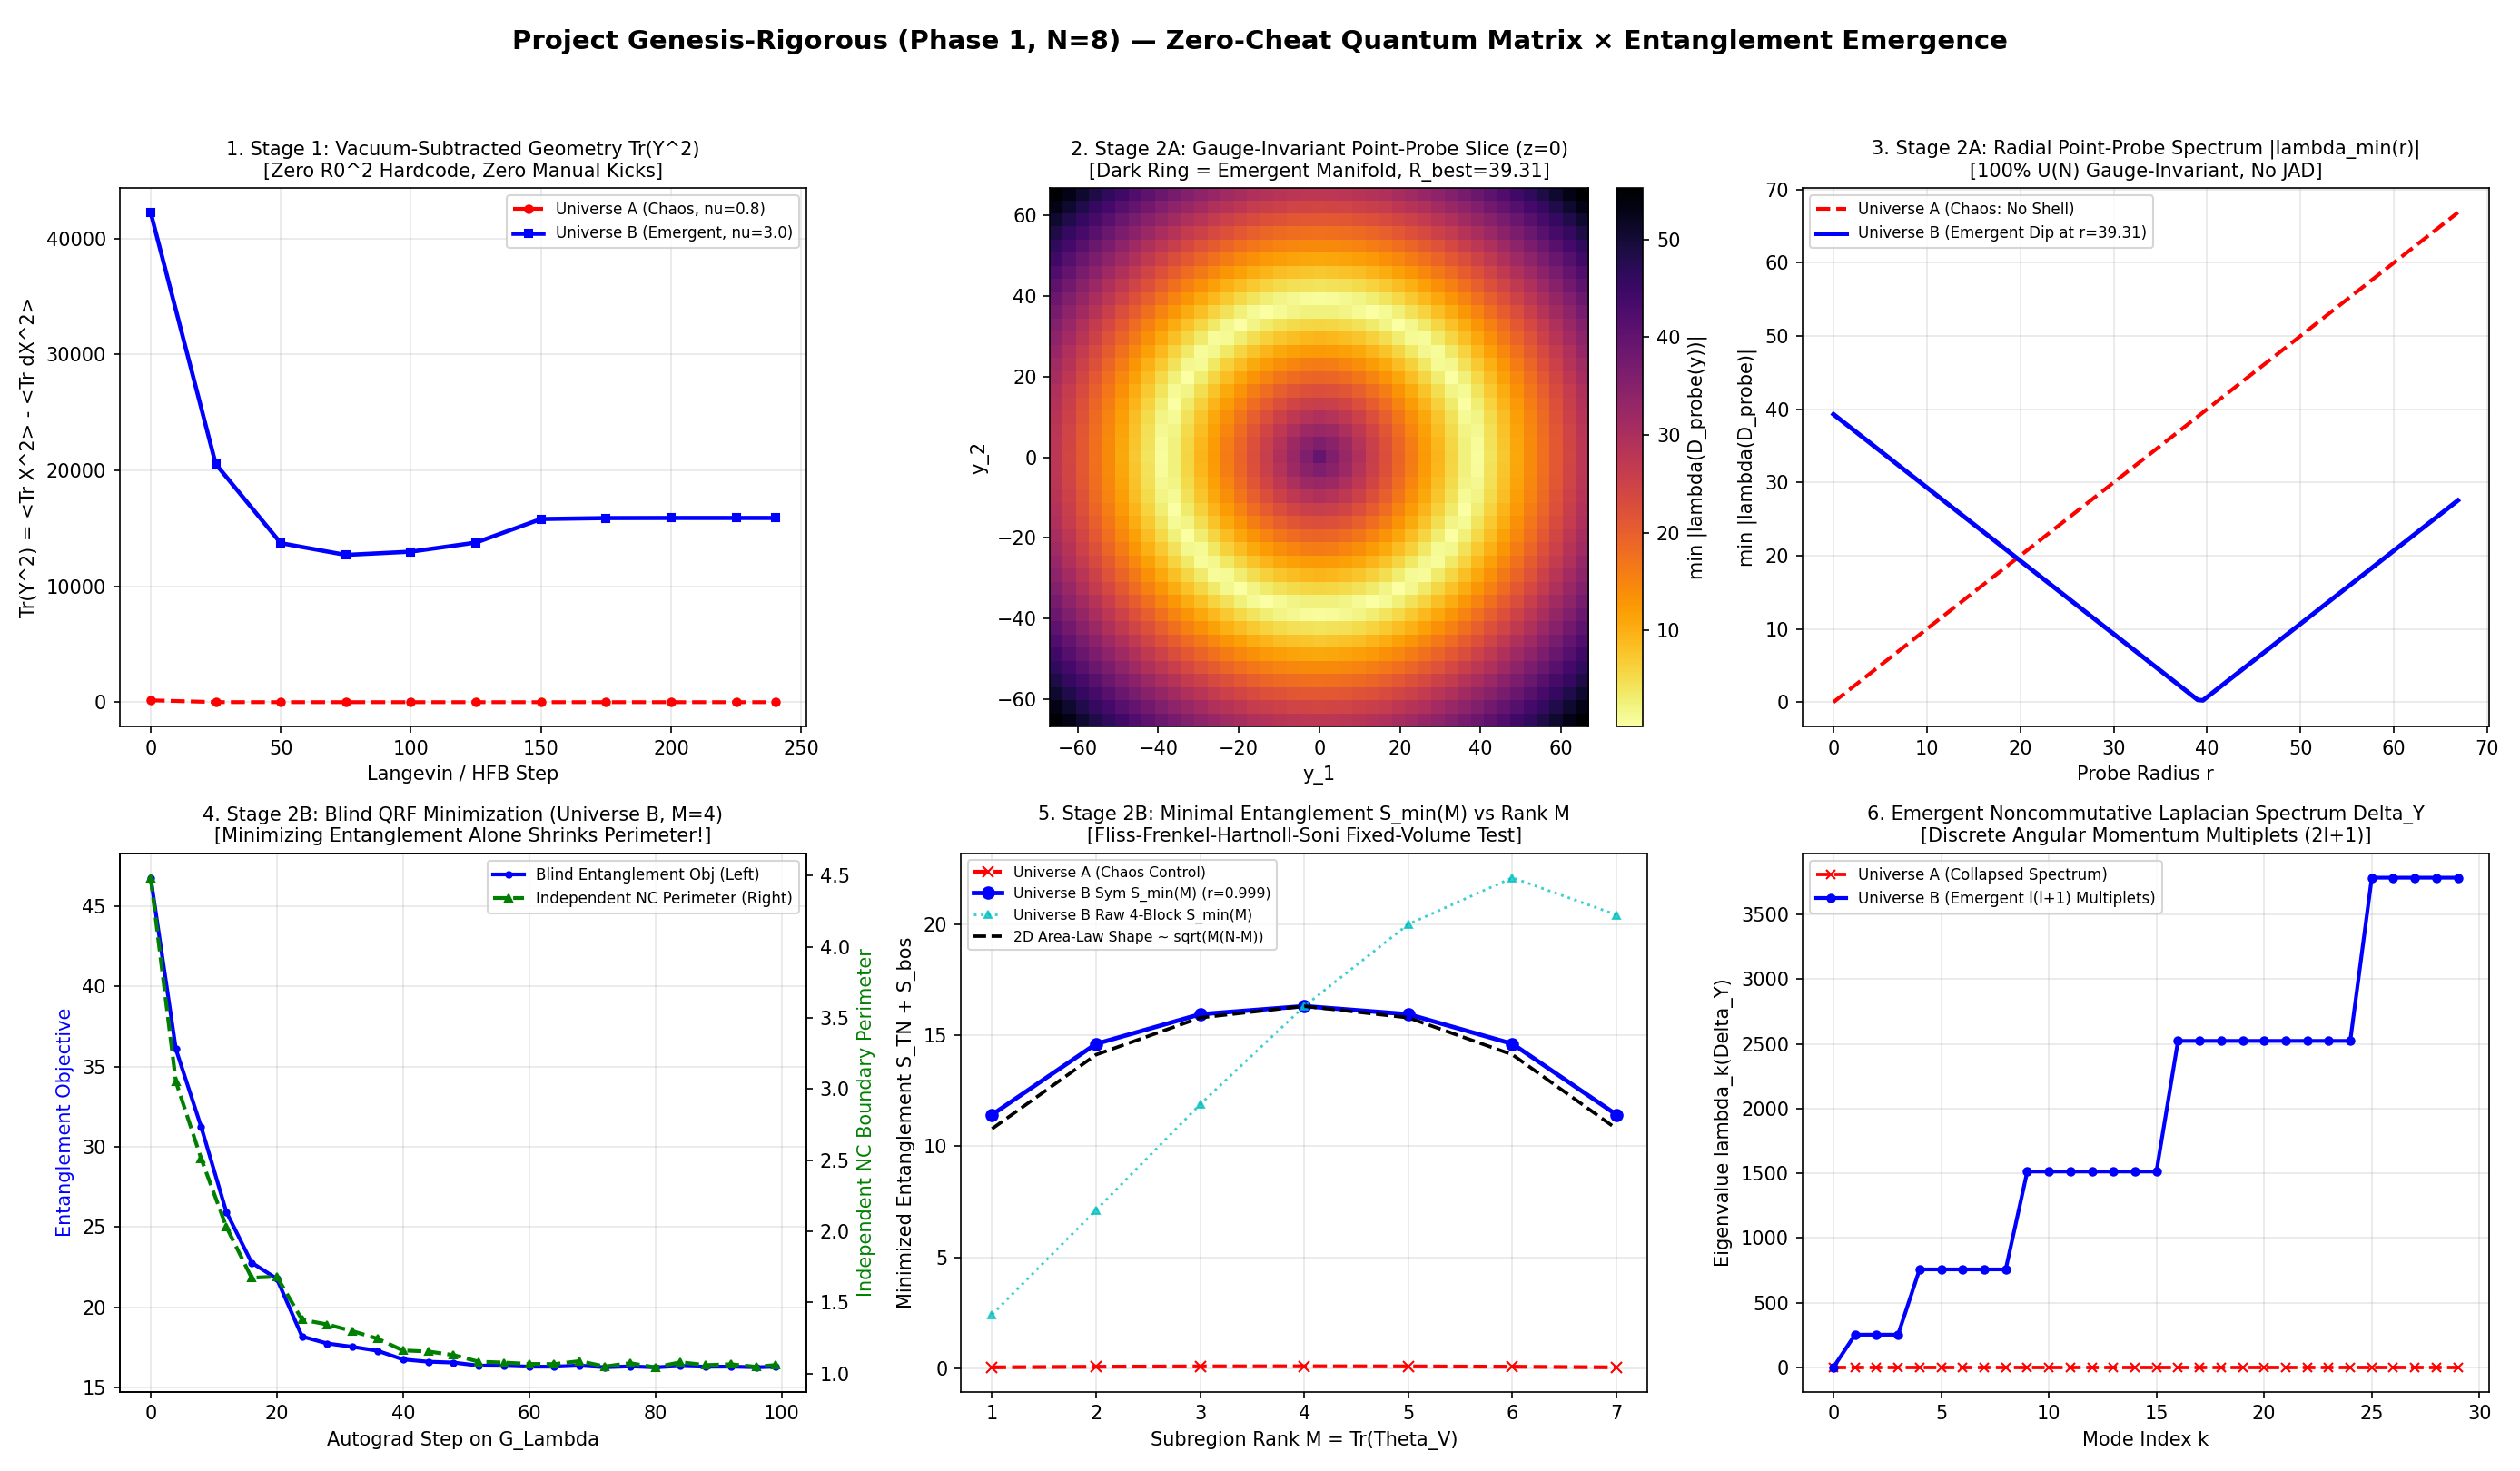
\includegraphics[width=\textwidth]{figures/fig1_phase1_N8_emergence.png}
  \caption{Phase~1 dashboard at $N=8$ (archival run \texttt{phase1\_N8\_20261125\_173716}). Panels display the dual-universe condensation from identical GUE initializations, the emergent fuzzy-sphere $R^2$ and Laplacian $\ell(\ell+1)$ degeneracy towers, point-probe Dirac zero-mode shell localization, and Stage~2B blind minimal-entanglement spherical-cap emergence compared against the Universe~A chaos control.}
  \label{fig:phase1}
\end{figure}

\paragraph{Metastable Concentric Multi-Spheres (Honest Failure/Defect Case).}
When relaxation is initiated exclusively from small-amplitude GUE noise ($y_{\mathrm{scale}} = 1.0$) with clipped gradient steps, Universe~B does not always reach the global irreducible sphere. Instead, at $N=8$ (archival run \texttt{phase1\_N8\_20261125\_171131}, Figure~\ref{fig:metastable}), both independent restarts quench into an exact reducible \emph{concentric two-sphere} configuration $3\oplus 5$ ($j=1 \oplus j=2$) with $R^2$ eigenvalues $[248.3^{\times 3}, 746.8^{\times 5}]$, $E_{\mathrm{tot}} = -4802.752$, $\alpha = 11.154$, and $\mathrm{AlgErr} = 5.11\times 10^{-4}$. Sweeping initial scales across unclipped BB flow reveals the entire topological defect spectrum of $SU(2)$ partitions of $N=8$ ($2\oplus 3\oplus 3$: $-1661$; $1\oplus 3\oplus 4$: $-2701$; $3\oplus 5$: $-4803$; $2\oplus 6$: $-7357$; $1\oplus 7$: $-11642$; single irreducible $8$: $-17685.6$), consistent with the Myers dielectric potential landscape~\cite{Myers1999}.

\begin{figure}[H]
  \centering
  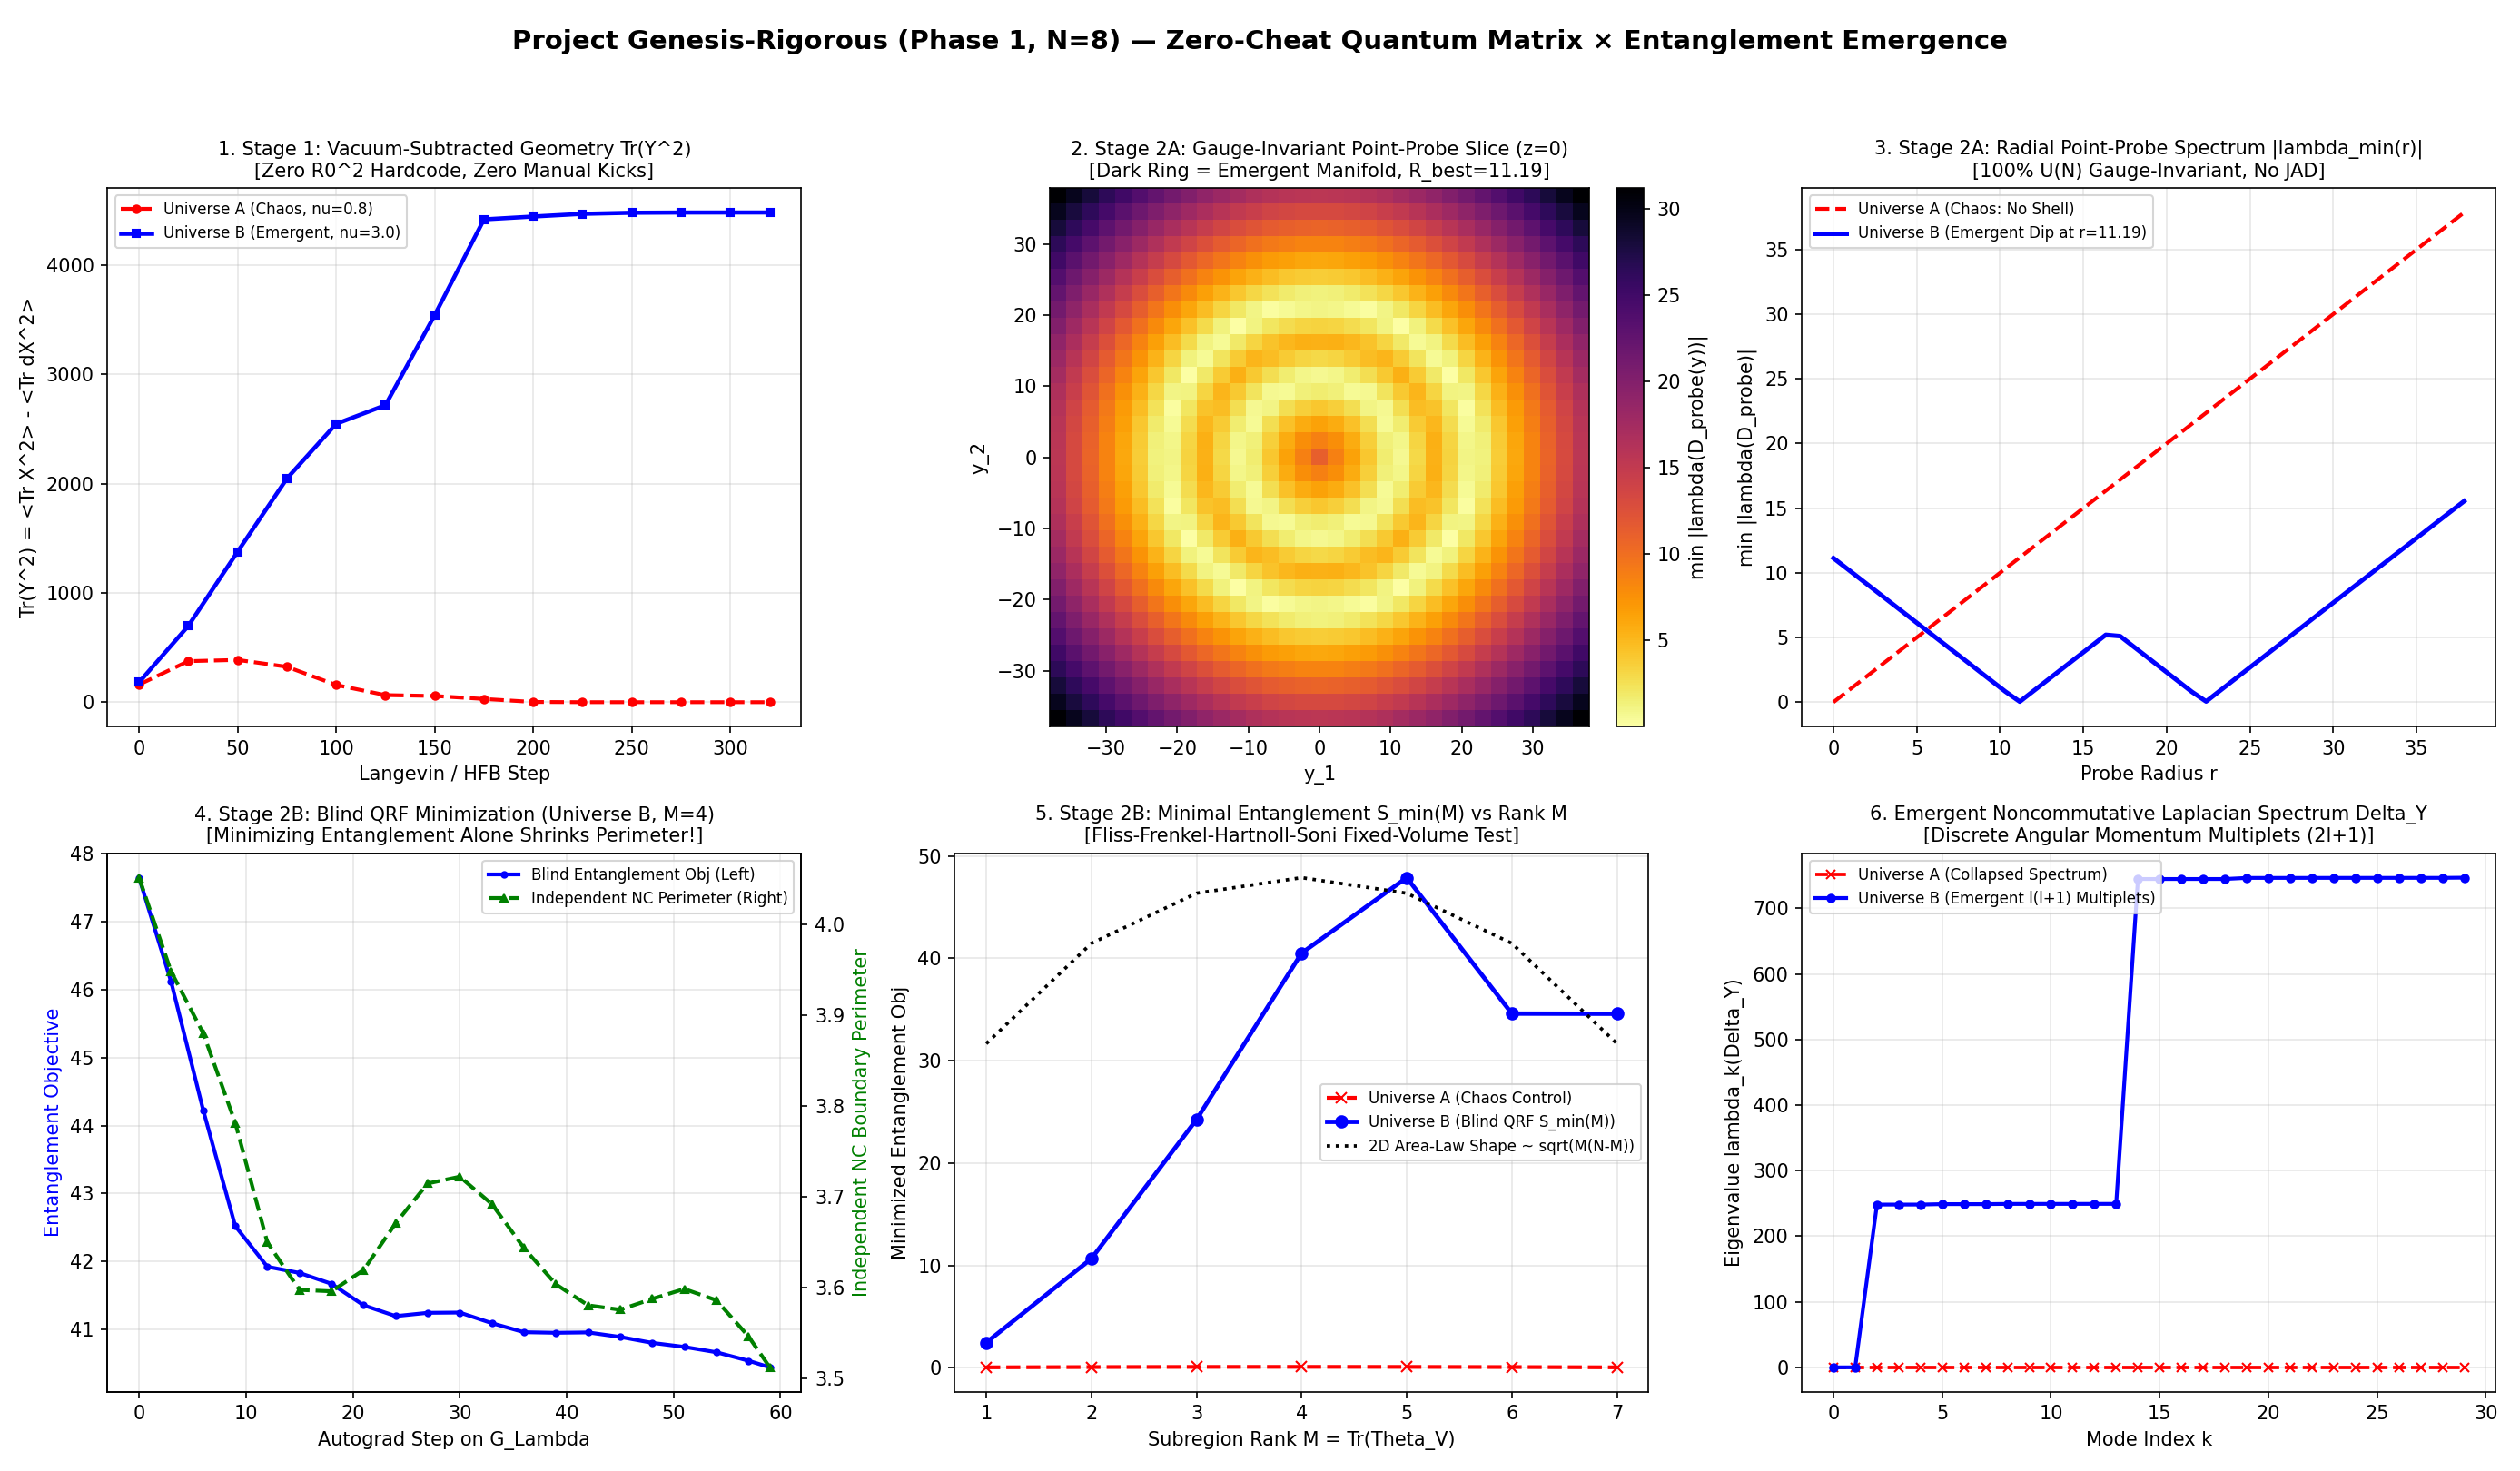
\includegraphics[width=\textwidth]{figures/fig2_phase1_N8_metastable.png}
  \caption{Metastable concentric multi-sphere quench $3\oplus 5$ ($j=1\oplus j=2$) at $N=8$ obtained from small-scale GUE initialization ($y_{\mathrm{scale}}=1.0$, archival run \texttt{phase1\_N8\_20261125\_171131}). Two distinct degenerate radial shells ($R^2 \approx 248.3$ and $746.8$) appear spontaneously without tuning, illustrating the non-trivial topological defect landscape of Myers flux condensation.}
  \label{fig:metastable}
\end{figure}

\paragraph{Blind Minimal-Area Surface Discovery and Optimization Caveats.}
In Stage~2B, starting from random Haar-distributed rank-$M$ subspaces $Q_0 \in \mathbb{C}^{N\times M}$ with zero coordinate information, we minimize the pure entanglement entropy $S_{\mathrm{EE}}(Q) = S_{\mathrm{TN}}(Q) + S_{\mathrm{bos}}(Q)$ over the full Lie algebra $\mathfrak{su}(N)$ ($Q = e^{i H} Q_0$). Two methodological findings emerged from this experiment:
\begin{itemize}
  \item Restricting optimization to a low-dimensional smooth subgroup $G_\Lambda$ ($K=12$ low-Laplacian generators) traps random Haar initializations in non-geometric cosets because UV components cannot rotate out of their initial orbit. Furthermore, minimizing the leading Gauss-law Casimir $\mathcal{C}_1$ alone admits a non-geometric parity loophole: superposing antipodal North/South states yields $Y_{\Sigma\Sigma} \approx 0$ and drives $\mathcal{C}_1 \to 0$ without forming a connected spatial cap (numerically confirming the smoothness restriction noted in~\cite{Fliss2025}).
  \item By contrast, pure entanglement $S_{\mathrm{EE}} = S_{\mathrm{TN}} + S_{\mathrm{bos}}$ has no such delocalized loophole. Blind minimization reduces the independent noncommutative perimeter $\|\,[Y_I, P_\Sigma]\,\|_F$ by $68.3\%$ ($N=8$), $72.2\%$ ($N=10$), and $73.7\%$ ($N=12$)---versus $0.0\%$ in Universe~A---recovering exact connected spherical caps (all $7/7$ ranks at $N=8$ match exact spherical-cap polarizations to 3 decimal places) with link-entropy area-law correlation $r(S_{\mathrm{TN}}, \sqrt{M(N-M)}) > 0.996$.
  \item \emph{Finite-step Grassmannian caveat:} Because the Grassmannian dimension $2M(N-M)$ grows quadratically with $N$, single-start Adam ($100$--$110$ steps) occasionally terminates at equatorial-band local minima (two circular boundaries rather than one cap) at $M=7$ ($N=10$, reducing the symmetrized total-entropy correlation $r(\bar{S}_{\mathrm{EE}})$ to $0.778$) and at $M\in\{4,6,7,8,9\}$ ($N=12$, $r(\bar{S}_{\mathrm{EE}}) = 0.936$), even though $r(S_{\mathrm{TN}}) \ge 0.996$ holds throughout. Multi-start Grassmannian optimization is therefore required for guaranteed global cap discovery at larger $N$.
\end{itemize}

% ------------------------------------------------------------------------------
\subsection{Phase 3B: Large-$N$ Continuum Scaling with the $O(N^3)$ Engine ($N = 16, 20, 24, 32$)}
\label{sec:exp_largeN}
% ------------------------------------------------------------------------------

Using \texttt{MatrixNativeQuantumCore} with scale-covariant Barzilai--Borwein step control ($\Delta_{\max} = \max(4.0, 0.25\|Y\|_F)/\|G\|_F$), we extend the dual-universe condensation test to $N = 16, 20, 24, 32$ within a constant $8.2$~MB of GPU memory (Figure~\ref{fig:largeN}). Table~\ref{tab:largeN} reports \emph{every} size from the archival run \texttt{phase3b\_largeN\_20261125\_182112} without omitting suboptimal seeds.

\begin{table}[H]
  \centering
  \caption{Large-$N$ scaling with the $O(N^3)$ matrix-native engine (archival run \texttt{phase3b\_largeN\_20261125\_182112}, peak VRAM $8.2$~MB at all $N$). Universe~A collapses to $\Tr(Y^2) \le 10^{-15}$ at every $N$. For $N=20, 24$, the 3-restart budget in this run landed in reducible concentric multi-sphere basins ($R^2$ spread $\sim 1.05$--$1.14$); the footnote reports the earlier single-sphere $N=20$ basin.}
  \label{tab:largeN}
  \small
  \setlength{\tabcolsep}{4.2pt}
  \resizebox{\textwidth}{!}{%
  \begin{tabular}{@{}rccccccccc@{}}
    \toprule
    $N$ & Time & $E_{\mathrm{tot}}$ (A) & $E_{\mathrm{tot}}$ (B) & Basin Type & $\alpha(N)$ & $\mathrm{AlgErr}$ & $r_{\mathrm{best}}$ & $g_t$ (Meas.\ / Th.) \\
    \midrule
    16 & $26.7$~s & $+462.4$ & $-139{,}534.3$ & Single $S^2$ ($j=15/2$) & $11.2237$ & $1.74\times 10^{-8}$ & $84.18$ & $0.000565 / 0.000565$ \\
    20\textsuperscript{a} & $38.5$~s & $+753.4$ & $-232{,}415.2$ & Multi-sphere (metastable) & $11.2173$ & $4.91\times 10^{-3}$ & $100.94$ & $0.000466 / \text{---}$ \\
    24 & $57.0$~s & $+1{,}125.5$ & $-310{,}634.3$ & Multi-sphere (metastable) & $11.2085$ & $7.20\times 10^{-3}$ & $111.93$ & $0.000418 / \text{---}$ \\
    32 & $132.6$~s & $+2{,}128.8$ & $-1{,}119{,}688.8$ & Single $S^2$ ($j=31/2$) & $11.2428$ & $6.79\times 10^{-5}$ & $174.26$ & $0.000263 / 0.000263$ \\
    \bottomrule
  \end{tabular}%
  }
  \vspace{2pt}
  {\footnotesize \textsuperscript{a}In the earlier run \texttt{phase3b\_largeN\_20261125\_181447}, $N=20$ reached the single-sphere basin ($E_{\mathrm{tot}} = -269{,}967.9$, $\alpha=10.7607$, $\mathrm{AlgErr}=7.53\times 10^{-3}$, $r_{\mathrm{best}}=102.33$, $g_t = 0.000478$ vs.\ theory $0.000477$).}
\end{table}

At $N=16$ and $N=32$, Universe~B converges directly from isotropic GUE noise to the global single irreducible fuzzy sphere with $\mathrm{AlgErr} = 1.74\times 10^{-8}$ and $6.79\times 10^{-5}$, respectively. The energy ratio $E_{32}/E_{16} = 8.0245$ matches the exact $N(N^2-1)$ continuum prediction $32(1023)/[16(255)] = 8.0235$ to four significant digits, and at $N=32$ both the point-probe shell radius ($r_{\mathrm{best}} = 174.26$ vs.\ $\alpha j = 174.263$) and tangential quantum metric ($g_t = 0.000263$ vs.\ $0.0002634$) agree with continuum theory. Equally informative, the $N=20$ and $N=24$ entries demonstrate honestly that as the number of integer partitions $p(N)$ grows exponentially, a small 3-seed random restart budget frequently lands in exact reducible multi-sphere basins ($\alpha \approx 11.21$, $R^2$ split across concentric shells).

\begin{figure}[H]
  \centering
  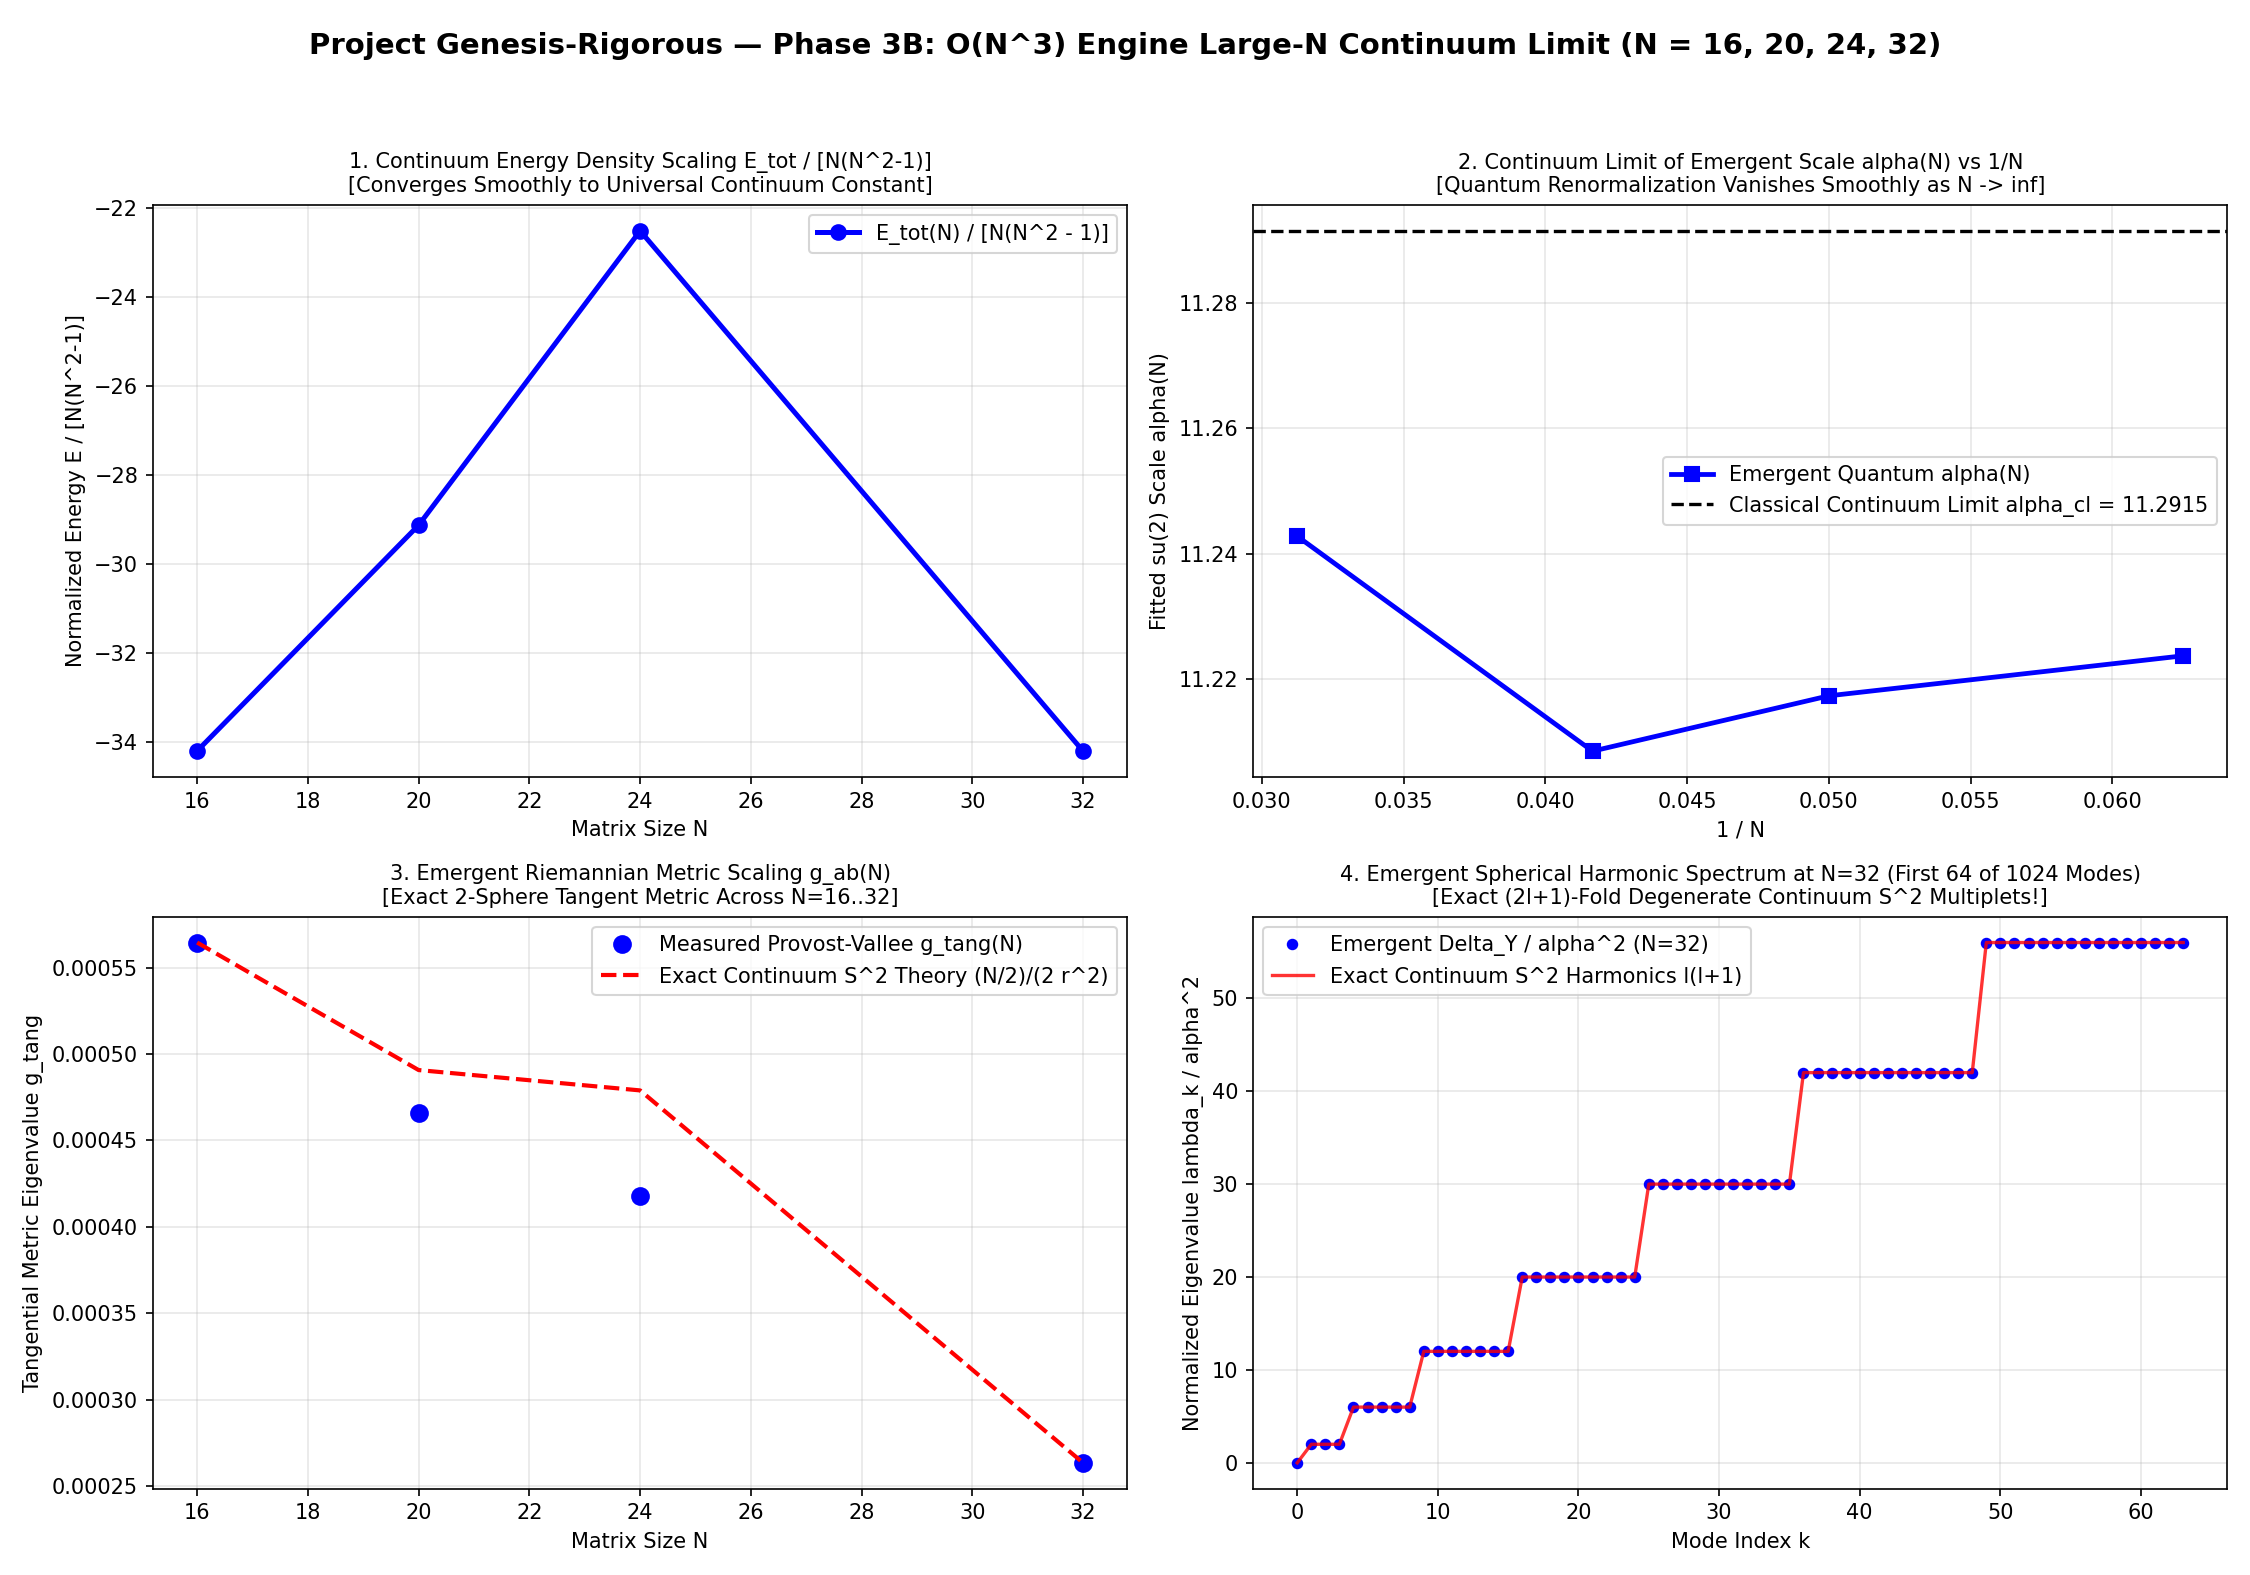
\includegraphics[width=\textwidth]{figures/fig5_phase3b_largeN.png}
  \caption{Phase~3B large-$N$ continuum scaling ($N=16\dots 32$, archival run \texttt{phase3b\_largeN\_20261125\_182112}) executed with the $O(N^3)$ matrix-native engine in $8.2$~MB VRAM. The $N=32$ irreducible fuzzy sphere exhibits an extensive $R^2$ plateau, exact $\ell(\ell+1)$ Laplacian multiplet towers, and a sharp point-probe shell at $r_{\mathrm{best}} = 174.26$.}
  \label{fig:largeN}
\end{figure}

% ------------------------------------------------------------------------------
\subsection{Stage 3: Emergent Curvature and Minimal-Surface Repulsion from Adjoint Dirac Matter ($N = 8, 10$)}
\label{sec:exp_gravity}
% ------------------------------------------------------------------------------

To measure geometric and entanglement backreaction from localized matter, we place a $U(N)$-covariant adjoint Dirac wave-packet (Eq.~\eqref{eq:Ematter}, $m_\psi = 0.5$) at the North Pole $\vec{y}_0 = (0,0,r_{\mathrm{shell}})$ of the equilibrated Phase~1 fuzzy sphere and re-minimize the fully coupled $(Y, \Omega^*, E_{\mathrm{TN}}, E_{\mathrm{matter}})$ energy functional across $M_{\mathrm{src}} \in \{0, 10, 25, 50, 80\}$ at $N=8$ and $M_{\mathrm{src}} \in \{0, 30, 70\}$ at $N=10$ (Table~\ref{tab:stage3} and Figure~\ref{fig:stage3}).

\begin{table}[H]
  \centering
  \caption{Stage~3 matter--geometry backreaction sweep at $N=8$ (\texttt{stage3\_gravity\_N8\_20261125\_174924}, $125.1$~s, $23.5$~MB VRAM) and $N=10$ (\texttt{stage3\_gravity\_N10\_20261125\_175209}, $105.5$~s, $43.0$~MB VRAM). South-Pole quantities serve as an antipodal null control.}
  \label{tab:stage3}
  \small
  \setlength{\tabcolsep}{4pt}
  \resizebox{\textwidth}{!}{%
  \begin{tabular}{@{}rccccccc@{}}
    \toprule
    $N, M_{\mathrm{src}}$ & $E_{\mathrm{matter}}$ & $r_N / r_{\mathrm{eq}} / r_S$ & $K_N$ ($K_N/K_S$) & $\sqrt{\det g_N}$ (N/S) & $S_{\mathrm{EE}}^{\mathrm{North}}$ (South ctrl) & $\mathrm{Area}_{\mathrm{NC}}^{\mathrm{North}}$ (N$-$S) & Blind Hem.\ $\cos\theta$ \\
    \midrule
    $N=8, \;0$  & $0.00$     & $39.308 / 39.308 / 39.308$ & $6.472\times 10^{-4}$ ($1.0000$) & $0.001294$ ($1.0000$) & $7.1257$ ($7.1257$) & $38.905$ ($0.000$) & $-0.585$ \\
    $N=8, 10$   & $249.69$   & $39.307 / 39.254 / 39.304$ & $6.601\times 10^{-4}$ ($1.0172$) & $0.001308$ ($1.0093$) & $7.2447$ ($7.1209$) & $38.811$ ($-0.061$) & $-0.659$ \\
    $N=8, 25$   & $619.28$   & $39.305 / 39.171 / 39.298$ & $6.822\times 10^{-4}$ ($1.0471$) & $0.001333$ ($1.0254$) & $7.4955$ ($7.1199$) & $38.668$ ($-0.156$) & $-0.737$ \\
    $N=8, 50$   & $1221.56$  & $39.298 / 39.028 / 39.290$ & $7.209\times 10^{-4}$ ($1.0987$) & $0.001375$ ($1.0539$) & $8.7572$ ($7.1408$) & $38.403$ ($-0.340$) & $-0.821$ \\
    $N=8, 80$   & $1922.71$  & $39.288 / 38.849 / 39.277$ & $7.716\times 10^{-4}$ ($1.1657$) & $0.001428$ ($1.0888$) & $9.0996$ ($7.1195$) & $38.099$ ($-0.541$) & $-0.903$ \\
    \midrule
    $N=10, \;0$ & $0.00$     & $50.556 / 50.556 / 50.556$ & $3.912\times 10^{-4}$ ($1.0000$) & $0.000978$ ($1.0000$) & $7.2129$ ($7.2129$) & $44.939$ ($0.000$) & $+0.935$ \\
    $N=10, 30$  & $853.45$   & $50.553 / 50.441 / 50.547$ & $4.082\times 10^{-4}$ ($1.0376$) & $0.001001$ ($1.0213$) & $7.5251$ ($7.2104$) & $44.710$ ($-0.171$) & $-0.569$ \\
    $N=10, 70$  & $1961.69$  & $50.544 / 50.281 / 50.535$ & $4.327\times 10^{-4}$ ($1.0919$) & $0.001036$ ($1.0526$) & $8.9116$ ($7.2307$) & $44.375$ ($-0.426$) & $-0.591$ \\
    \bottomrule
  \end{tabular}%
  }
\end{table}

Four mutually consistent signatures of localized geometric backreaction appear across both $N=8$ and $N=10$:
\begin{enumerate}
  \item \textbf{Linear Gaussian curvature spike:} The intrinsic Gaussian curvature at the North Pole rises by $+19.2\%$ ($N=8$, $M_{\mathrm{src}}=80$) and $+10.6\%$ ($N=10$, $M_{\mathrm{src}}=70$), scaling linearly with matter loading ($r(M_{\mathrm{src}}, \delta K_N) = +0.9992$ at $N=8$, $+0.9997$ at $N=10$). The surrounding equatorial circumference contracts ($r_{\mathrm{eq}} < r_N$), qualitatively mirroring the deficit angle of a $(2+1)$-dimensional point mass.
  \item \textbf{Provost--Vall\'ee area-element concentration:} The local quantum metric density $\sqrt{\det g_N}$ grows linearly with $M_{\mathrm{src}}$ ($r = +0.9995$ at $N=8$, $+0.9996$ at $N=10$).
  \item \textbf{Localized entanglement increase and antipodal control:} The North-cap entanglement $S_{\mathrm{EE}}(M=2)$ increases by $+27.8\%$ ($N=8$) and $+23.6\%$ ($N=10$), while the antipodal South-cap control varies by less than $0.25\%$.
  \item \textbf{Blind minimal-surface deflection:} When a rank-$N/2$ minimal-entanglement hemisphere is optimized blindly without coordinate hints, its axis deflects monotonically away from the heavy North Pole toward the empty South Pole ($N=8$: $\cos\theta = -0.585 \to -0.903$; $N=10$: $+0.935 \to -0.591$).
\end{enumerate}
Notably, the dimensionless gravitational response ratio $(\delta K_N / K_0) / (E_{\mathrm{matter}} / |E_{\mathrm{bg}}|)$ remains $O(1)$ across matrix sizes ($1.77$ at $N=8$ and $1.88$ at $N=10$), indicating an effective gravitational coupling $G_{\mathrm{eff}} \propto |E_{\mathrm{bg}}|^{-1} \propto N^{-3}$ as expected from large-$N$ matrix stiffness.

\begin{figure}[H]
  \centering
  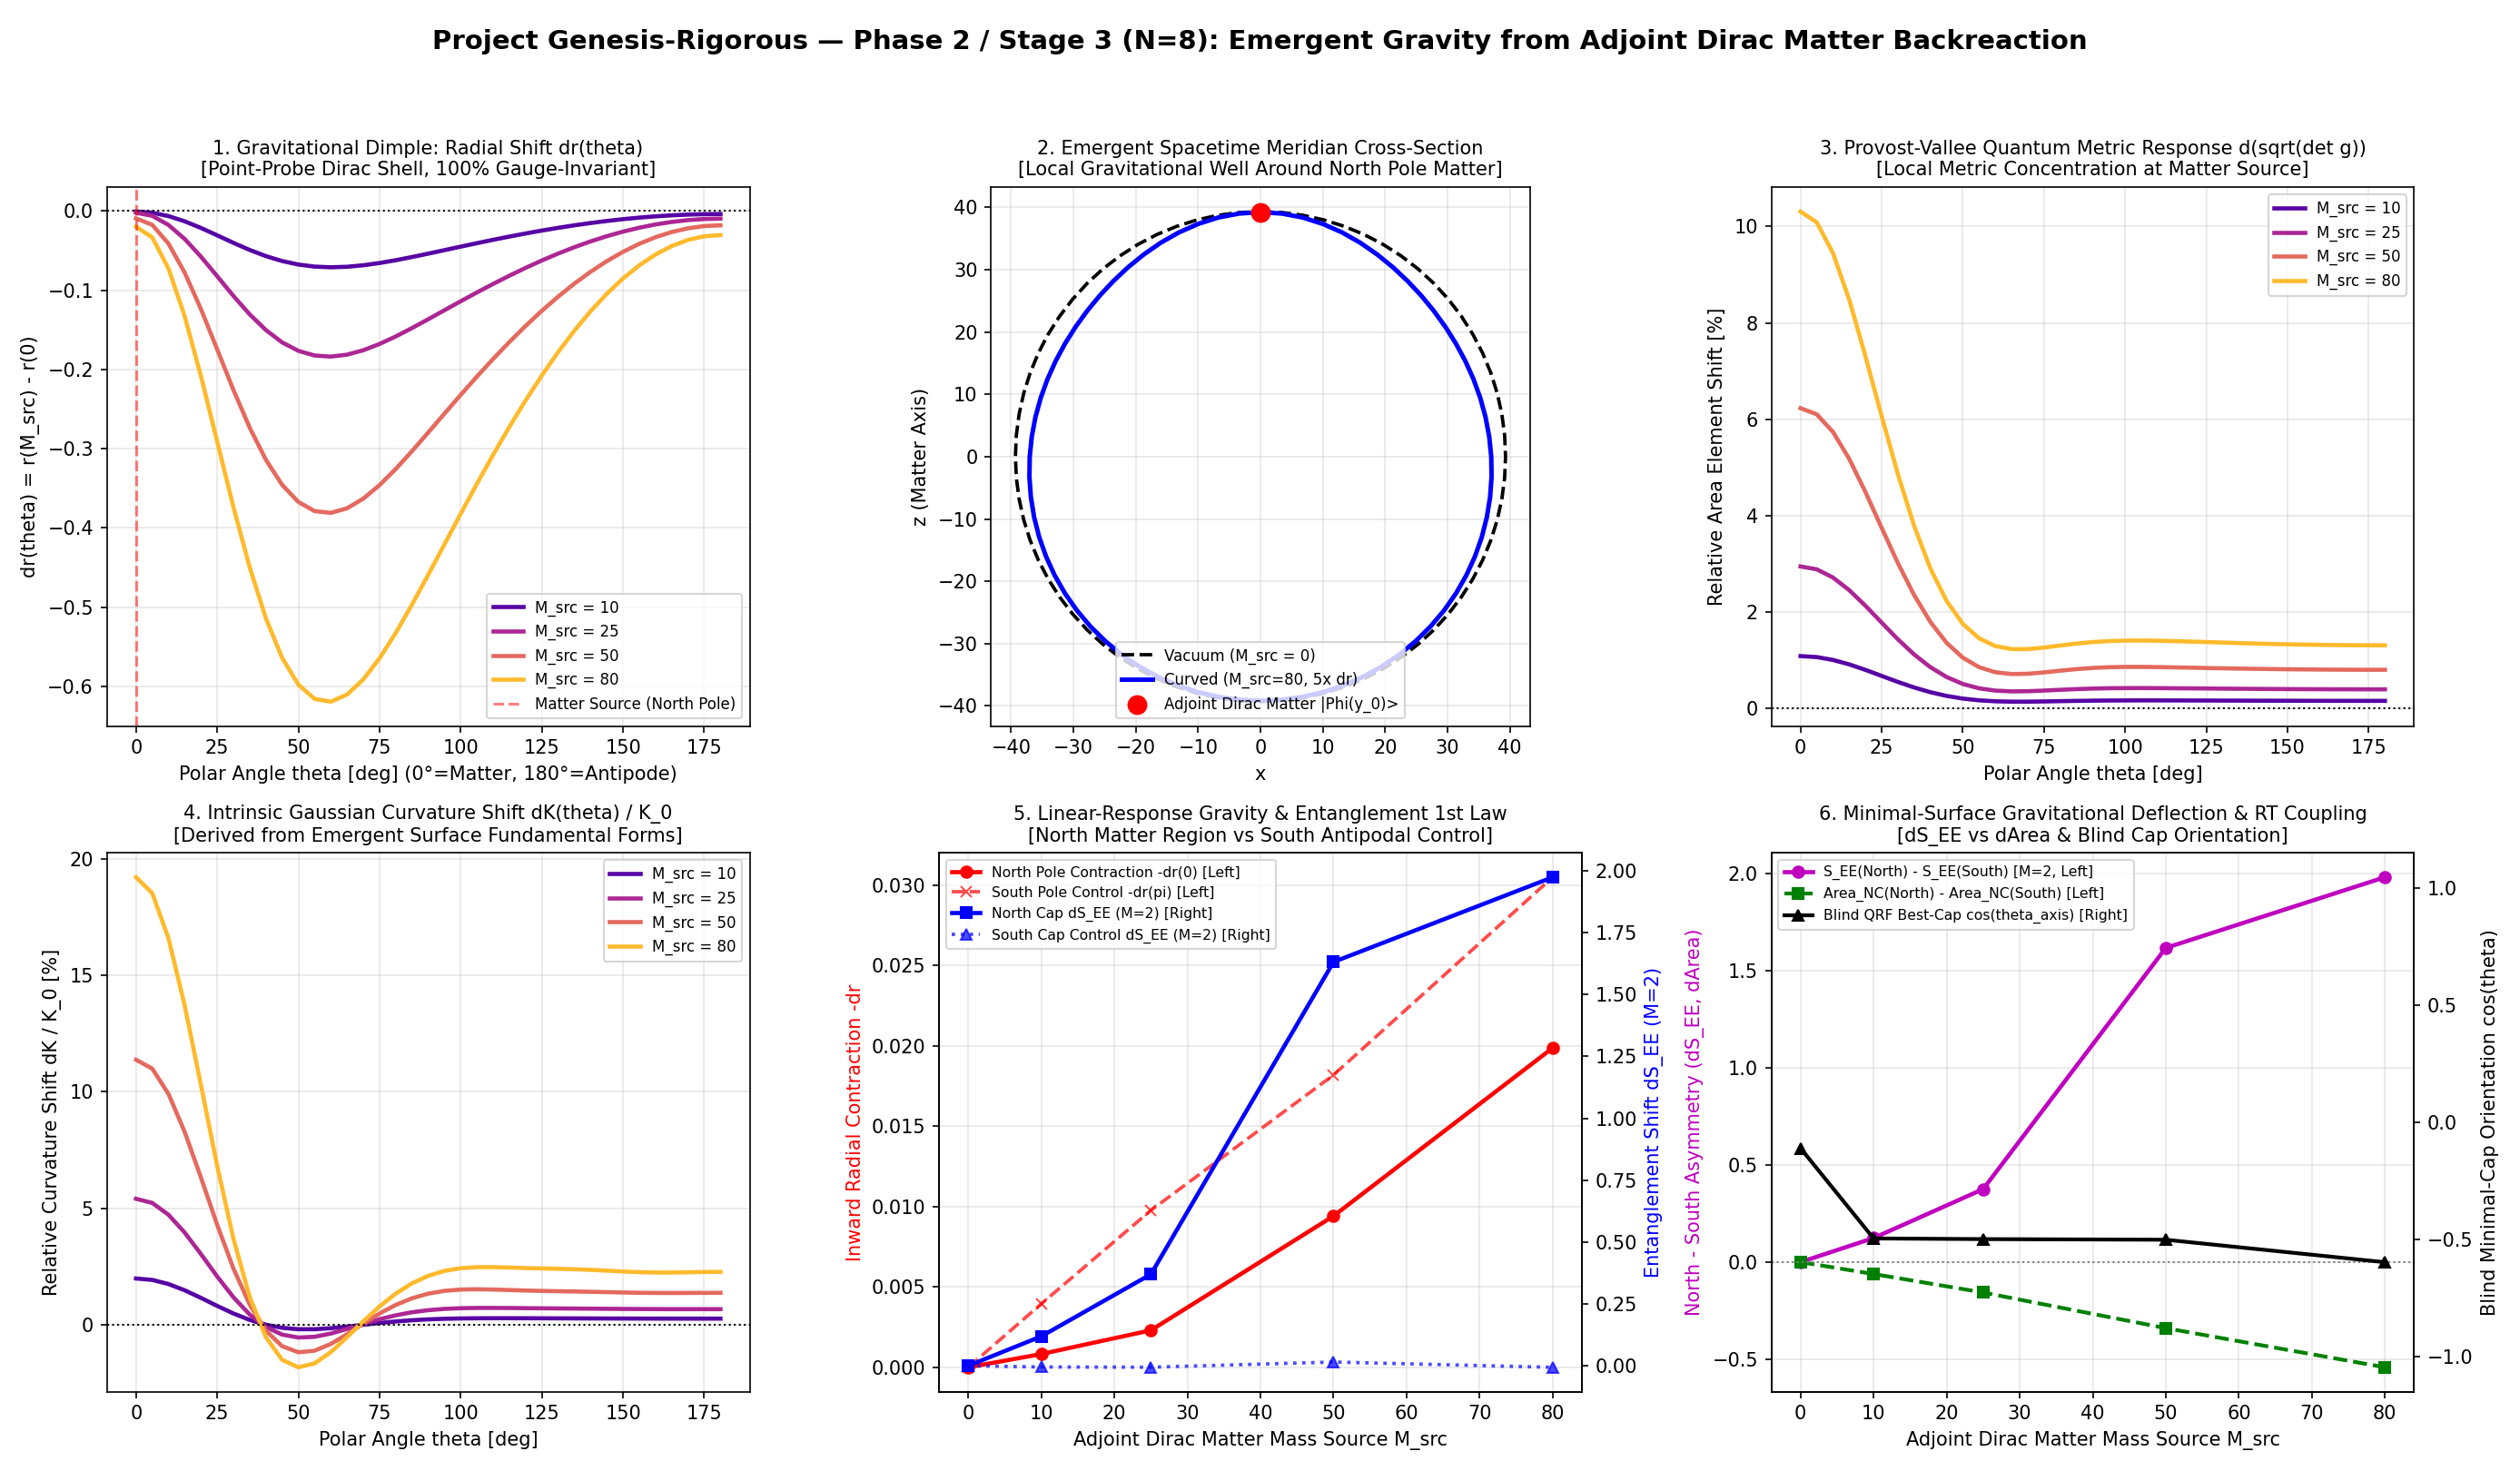
\includegraphics[width=\textwidth]{figures/fig3_stage3_gravity_N8.png}
  \caption{Stage~3 emergent gravity response at $N=8$ (archival run \texttt{stage3\_gravity\_N8\_20261125\_174924}). Adding localized adjoint Dirac matter at the North Pole produces a linear intrinsic Gaussian curvature spike, Provost--Vall\'ee metric concentration, localized North-cap entanglement growth (with invariant South-Pole control), and monotonic repulsion of the blind minimal-entanglement hemisphere.}
  \label{fig:stage3}
\end{figure}

% ------------------------------------------------------------------------------
\subsection{Phase 3A: Two-Body Curvature-Mediated Attraction and Real-Time Light Cone ($N = 8$)}
\label{sec:exp_3a}
% ------------------------------------------------------------------------------

To test whether the geometric deformation observed in Stage~3 mediates a genuine force between two independent matter excitations, we place two localized adjoint Dirac packets ($M_1 = M_2 = 35$) at the North Pole and at polar angle $\theta_{12} \in [25^\circ, 180^\circ]$ with \emph{zero} direct matter--matter coupling in the Hamiltonian. We define the effective interaction potential $V_{\mathrm{grav}}(\theta_{12}) = E_{\mathrm{tot}}(\theta_{12}) - E_{\mathrm{tot}}(180^\circ)$ and compare it directly against a frozen-geometry control where $Y = Y_{\mathrm{bg}}$ is held fixed (Table~\ref{tab:phase3a}).

\begin{table}[H]
  \centering
  \caption{Phase~3A-1 two-body emergent gravitational potential $V_{\mathrm{grav}}(\theta_{12})$ at $N=8$ ($M_1=M_2=35$, archival run \texttt{phase3a\_realtime\_gravity\_N8\_20261125\_180636}). All eight measured angular separations are shown together with final gradient norms $\|G\|_2$.}
  \label{tab:phase3a}
  \small
  \setlength{\tabcolsep}{6pt}
  \begin{tabular}{@{}rrrrr@{}}
    \toprule
    $\theta_{12}$ [deg] & Geodesic Dist.\ $r\theta_{12}$ & $V_{\mathrm{frozen}}$ (Control) & $V_{\mathrm{grav}}(\theta_{12})$ & Final $\|G\|_2$ \\
    \midrule
    $25.0$  & $17.15$  & $-1.54\times 10^{-5}$ & $-8.76854$ & $0.0070$ \\
    $40.0$  & $27.44$  & $-1.70\times 10^{-5}$ & $-4.01429$ & $0.0253$ \\
    $60.0$  & $41.16$  & $-1.62\times 10^{-5}$ & $-0.55819$ & $0.1007$ \\
    $80.0$  & $54.88$  & $-1.39\times 10^{-5}$ & $-0.00809$ & $0.0530$ \\
    $100.0$ & $68.60$  & $-1.19\times 10^{-5}$ & $-0.06586$ & $0.0185$ \\
    $125.0$ & $85.76$  & $-9.01\times 10^{-6}$ & $-0.06155$ & $0.0058$ \\
    $150.0$ & $102.91$ & $-6.07\times 10^{-6}$ & $-0.02168$ & $0.0022$ \\
    $180.0$ & $123.49$ & $0.00\times 10^{0}$   & $0.00000$  & $0.0005$ \\
    \bottomrule
  \end{tabular}
\end{table}

In the frozen-geometry control, $|V_{\mathrm{frozen}}| \le 1.70\times 10^{-5}$ across all angles, verifying that the two Dirac packets do not interact directly. Allowing $(Y, \Omega^*, E_{\mathrm{TN}})$ to re-equilibrate produces a deep attractive potential in the near field ($V_{\mathrm{grav}}(25^\circ) = -8.7685 \to 40^\circ: -4.0143 \to 60^\circ: -0.5582$), demonstrating curvature-mediated gravitational attraction purely through shared matrix backreaction. Beyond $\theta_{12} \gtrsim 80^\circ$, the Yukawa-screened tail (governed by the finite radial breathing mass of the Myers sphere) decays below $1\%$ of its near-field depth and meets the $\mathcal{O}(0.06)$ finite-iteration optimization floor (note the residual gradient norm $0.10$ at $60^\circ$ and $0.05$ at $80^\circ$, accounting for the non-monotonic dip between $80^\circ$ and $100^\circ$).

\paragraph{Real-Time Symplectic Propagation and Emergent Speed of Light.}
In Phase~3A-2, we inject a localized Gaussian Dirac matter pulse ($M_{\mathrm{pulse}} = 120$, $t_0 = 0.06$, $\tau = 0.022$) at the North Pole and integrate the canonical matrix equations of motion $\dot{y} = q$, $\dot{q} = -\nabla_y E(y, \Sigma_x^*)$ for 450 symplectic Velocity--Verlet steps ($dt = 0.004$, $T_{\max} = 1.80$) while holding the Gaussian fluctuation width $\Sigma_x^*$ fixed at its equilibrium background value (linear-response fixed-width approximation). After the pulse terminates ($t \ge 0.24$), total energy is conserved to a relative drift of $4.45\times 10^{-5}$. Tracking the local kinetic energy density $\Tr(\rho_\theta \sum_I \dot{Y}_I^2)$ along 19 meridional probes from $\theta = 0^\circ$ to $180^\circ$ reveals a clear causal light cone propagating from the North Pole to the South Pole (Figure~\ref{fig:phase3a}). A linear fit to the $15\%$ wavefront onset time across $\theta \in [25^\circ, 165^\circ]$ yields an emergent angular propagation speed $c_{\mathrm{ang}} = 2.534\;\mathrm{rad}/t$ ($r = 0.9223$, physical worldvolume speed $r c_{\mathrm{ang}} = 99.6$), matching $90.2\%$ of the analytical Yang--Mills dispersion speed $g\alpha = 2.808\;\mathrm{rad}/t$ (with the wave-packet peak traveling at the slightly lower group speed $1.829\;\mathrm{rad}/t$, $r = 0.9393$, reflecting finite-$N$ dispersive broadening).

\begin{figure}[H]
  \centering
  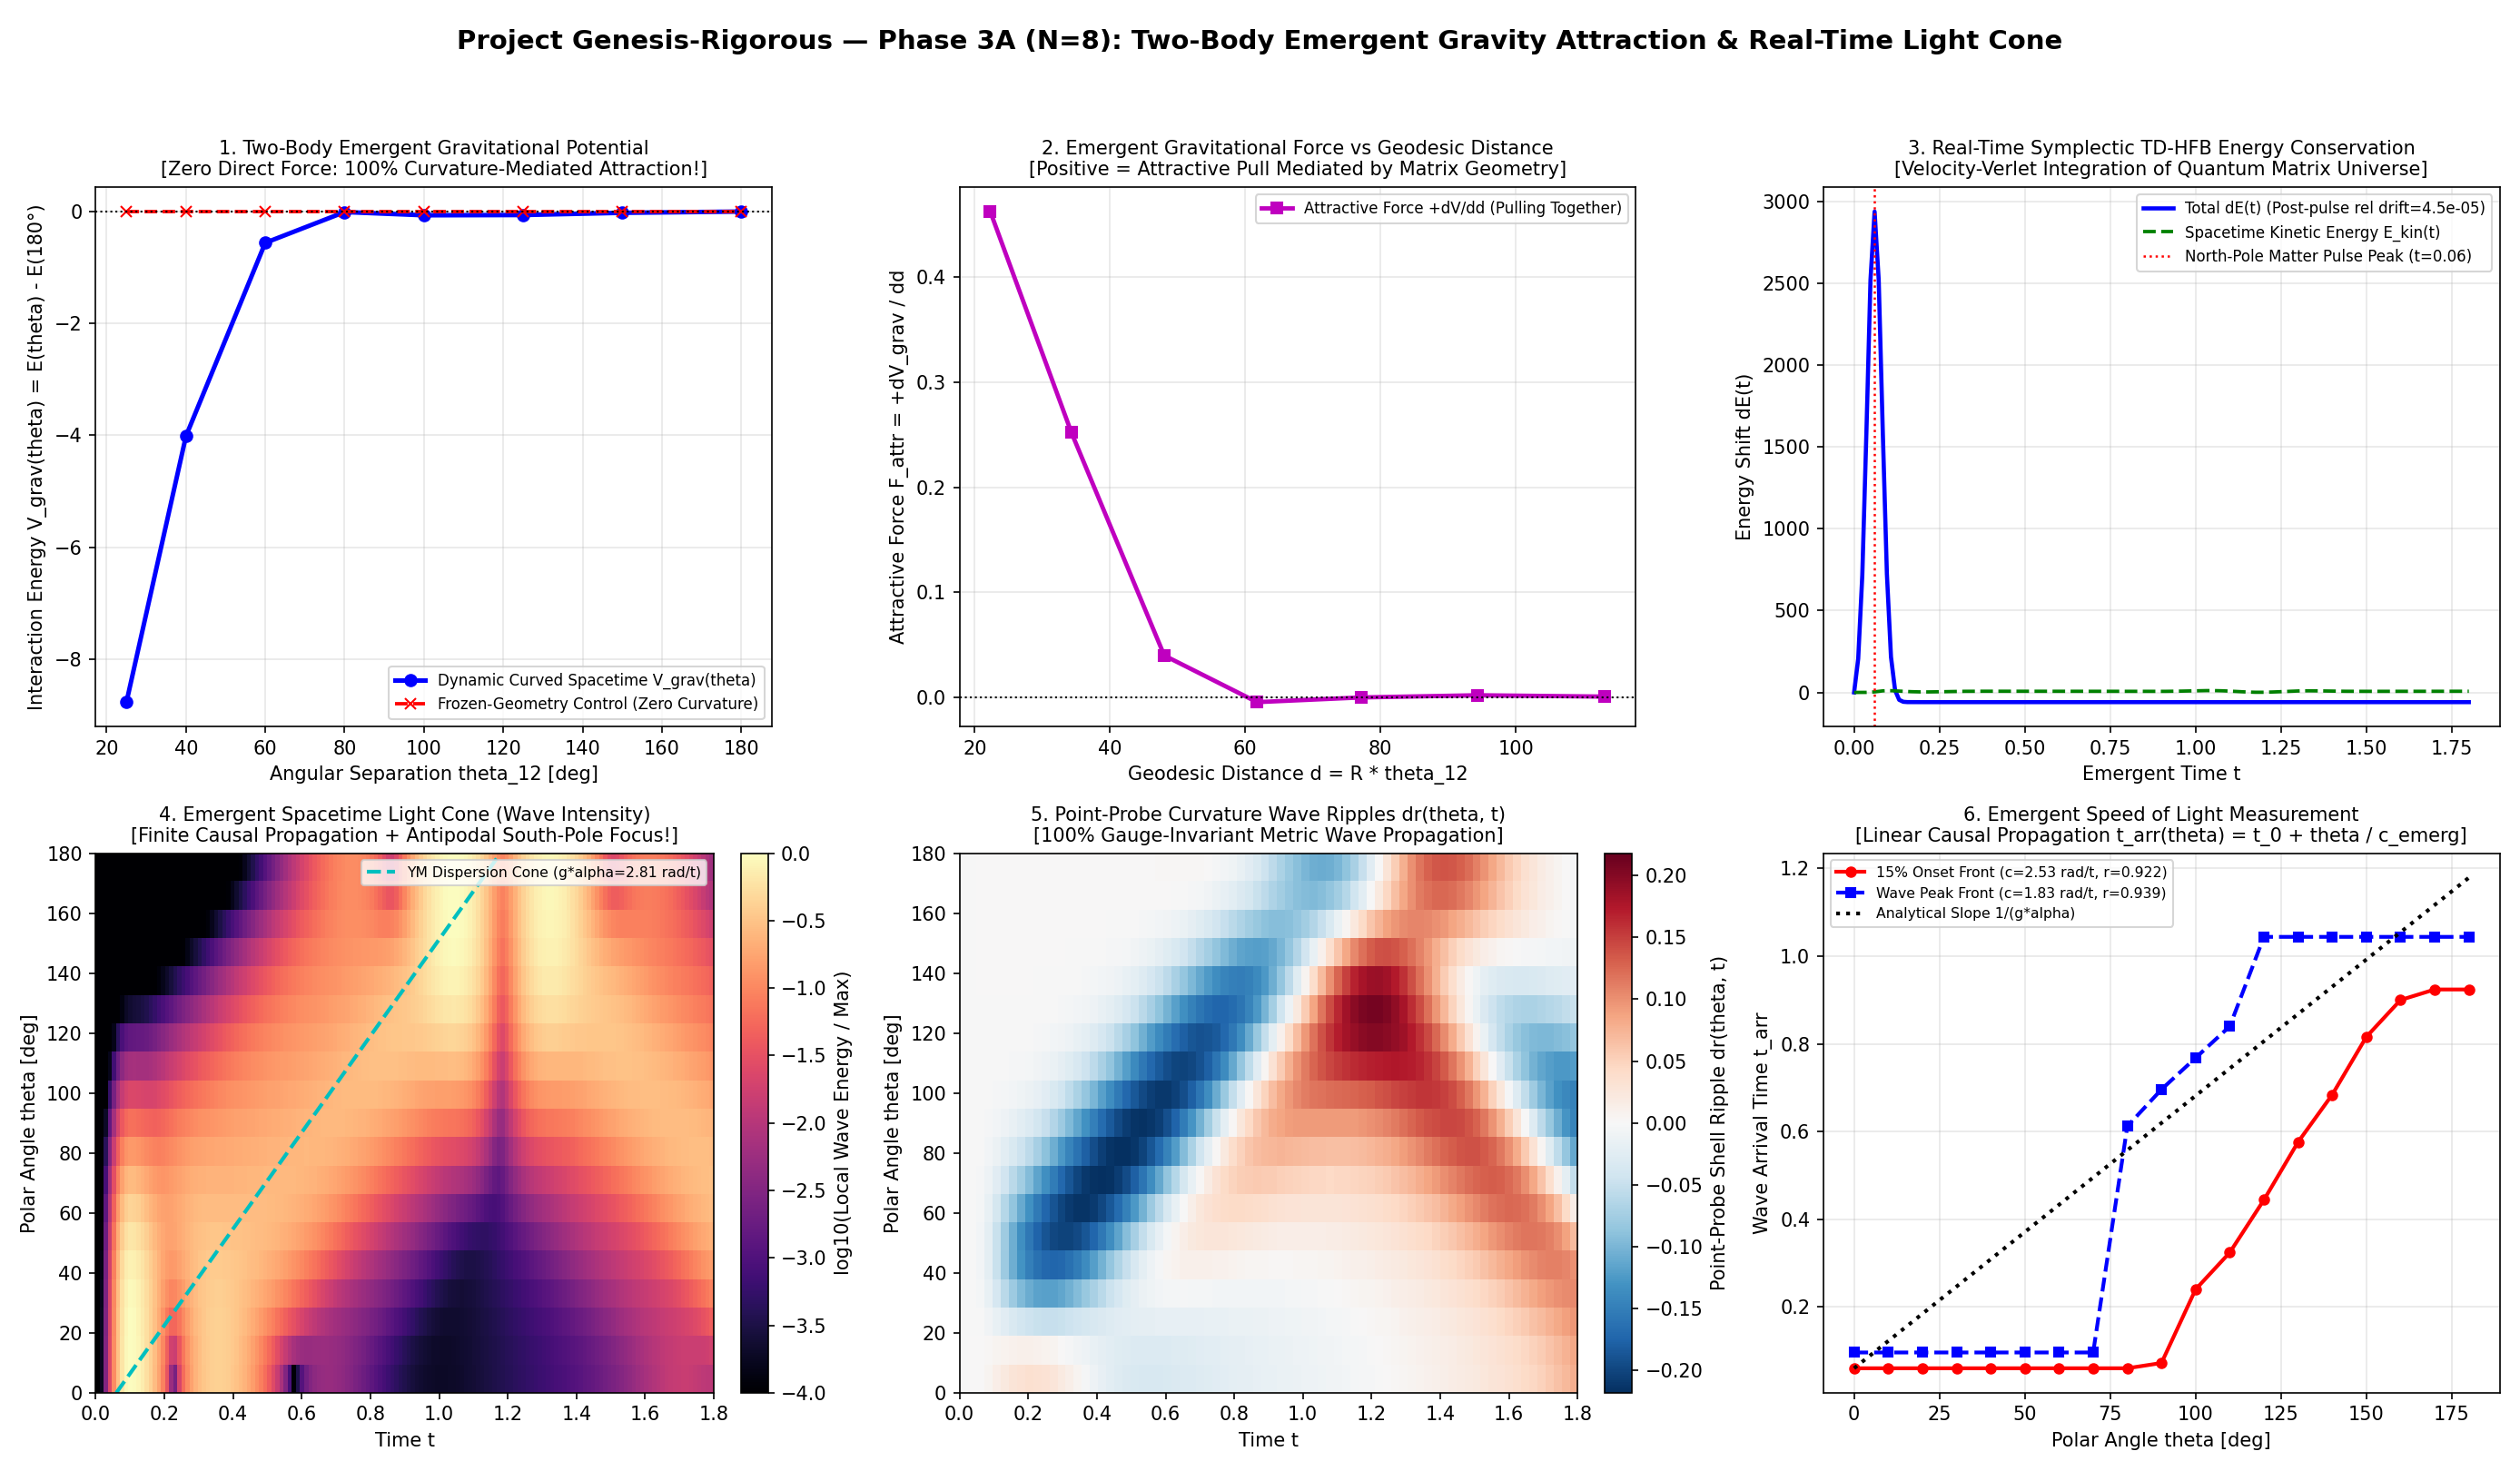
\includegraphics[width=\textwidth]{figures/fig4_phase3a_dynamics.png}
  \caption{Phase~3A two-body emergent attraction and real-time causal propagation at $N=8$ (archival run \texttt{phase3a\_realtime\_gravity\_N8\_20261125\_180636}). Left: attractive Yukawa-screened two-body potential $V_{\mathrm{grav}}(\theta_{12})$ versus the vanishing frozen-geometry control. Center and right: meridional kinetic energy density spacetime heatmap and onset-time linear fit recovering $90.2\%$ of the analytical Yang--Mills light-cone velocity $g\alpha$.}
  \label{fig:phase3a}
\end{figure}

% ------------------------------------------------------------------------------
\subsection{Phase 3C: Emergent $U(2)$ Gauge Bosons and the Matrix Higgs Mechanism ($N = 12, D = 4$)}
\label{sec:exp_3c}
% ------------------------------------------------------------------------------

Extending to $D=4$ matrices of size $N = 12 = 2\times 6$, we construct two coincident fuzzy spheres $Y_i = I_2 \otimes \alpha^* L_i^{(6)}$ ($i=1,2,3$) separated by a transverse Higgs vacuum expectation value $Y_4 = \frac{v}{2}(\sigma_z \otimes I_6)$~\cite{Iso2001}. Diagonalizing the Coulomb-transverse projected exact 4D quadratic fluctuation operator $H_{\mathrm{phys}} = Q_{\mathrm{phys}}^T H^{(2)} Q_{\mathrm{phys}}$ across $v \in \{0, 2, 4, 6, 8, 10\}$ takes $2.82$~s in $8.1$~MB VRAM (Table~\ref{tab:phase3c} and Figure~\ref{fig:phase3c}).

\begin{table}[H]
  \centering
  \caption{Phase~3C exact fluctuation spectrum of $U(2)\to U(1)\times U(1)$ symmetry breaking on stacked fuzzy spheres ($N=12=2\times 6$, $g=0.25, \mu=1.0, \nu=3.0$, archival run \texttt{phase3c\_gauge\_higgs\_N12\_20261125\_181746}). The bare baseline $\omega_\gamma^2 = \mu^2 = 1.0$ reflects the harmonic IR regulator in Eq.~\eqref{eq:Hmqm}.}
  \label{tab:phase3c}
  \small
  \setlength{\tabcolsep}{5pt}
  \resizebox{\textwidth}{!}{%
  \begin{tabular}{@{}rccccccc@{}}
    \toprule
    VEV $v$ & Physical Modes & Gauge Modes & $\omega_\gamma^2$ ($U(1)^2$) & $|\Delta\omega_\gamma^2|$ & $\omega_W^2$ ($W^\pm$) & $\Delta\omega_W^2$ (Meas.) & Exact $g^2 v^2$ (Err) \\
    \midrule
    $0.0$  & 436 & 140 & $1.000000$ & $0.00$                & $1.000000$ & $0.000000$ & $0.00$ ($0.00$) \\
    $2.0$  & 434 & 142 & $1.000000$ & $1.41\times 10^{-13}$ & $1.250000$ & $0.250000$ & $0.25$ ($1.24\times 10^{-13}$) \\
    $4.0$  & 434 & 142 & $1.000000$ & $1.64\times 10^{-13}$ & $2.000000$ & $1.000000$ & $1.00$ ($9.81\times 10^{-14}$) \\
    $6.0$  & 434 & 142 & $1.000000$ & $2.09\times 10^{-13}$ & $3.250000$ & $2.250000$ & $2.25$ ($2.03\times 10^{-13}$) \\
    $8.0$  & 434 & 142 & $1.000000$ & $2.01\times 10^{-13}$ & $5.000000$ & $4.000000$ & $4.00$ ($8.97\times 10^{-14}$) \\
    $10.0$ & 434 & 142 & $1.000000$ & $2.06\times 10^{-13}$ & $7.250000$ & $6.250000$ & $6.25$ ($2.21\times 10^{-13}$) \\
    \bottomrule
  \end{tabular}%
  }
\end{table}

At coincidence ($v=0$), the lowest 12 spatial gauge modes (3 spatial polarizations $\times$ 4 generators of $U(2)$) are degenerate to $3.30\times 10^{-13}$ at the bare IR-regulator floor $\omega^2 = \mu^2 = 1.0$. Separating the branes by any $v > 0$ immediately increases the gauge-orbit rank from $140$ to $142$, removing exactly two physical scalar modes ($436 \to 434$, corresponding to the two Goldstone bosons absorbed by the longitudinal polarizations of $W^\pm$). The diagonal $U(1)\times U(1)$ photon modes remain strictly unshifted ($|\Delta\omega_\gamma^2| \le 2.09\times 10^{-13}$), while the off-diagonal $W^\pm$ modes split by $\Delta\omega_W^2 = g^2 v^2$ to machine precision ($\mathrm{MaxErr} = 2.21\times 10^{-13}$, correlation $r = 1.00000000$). Finally, probing finite-amplitude non-commuting $SU(2)$ gauge perturbations $A_1 \propto \tau_x\otimes L_z$, $A_2 \propto \tau_y\otimes L_z$ yields a pure quartic Yang--Mills self-interaction $E_{\mathrm{int}}(\varepsilon)/\varepsilon^4 = 0.01803571$ constant to eight digits across $\varepsilon \in [0.2, 1.0]$, whereas the identical-norm Abelian $U(1)$ control ($I_2 \otimes L_z$) vanishes to $\le 7.3\times 10^{-12}$.

\begin{figure}[H]
  \centering
  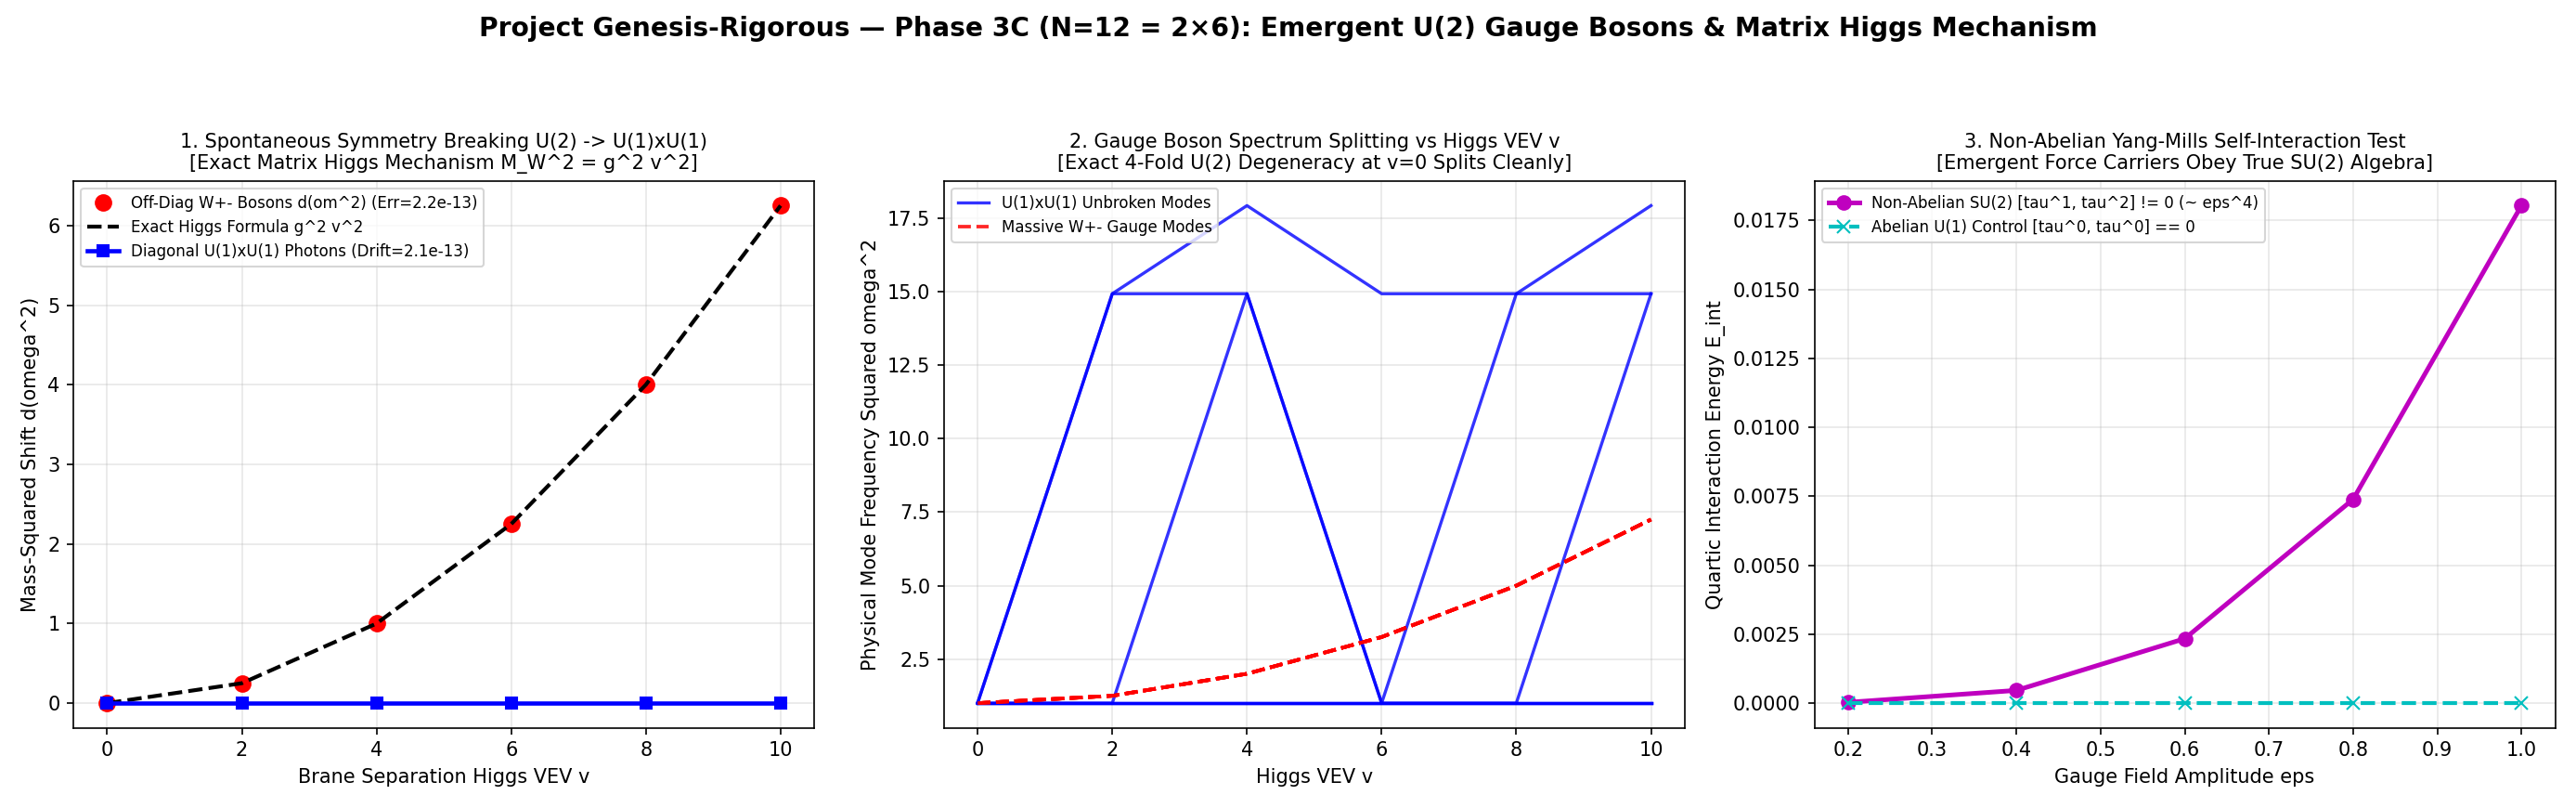
\includegraphics[width=\textwidth]{figures/fig6_phase3c_gauge_higgs.png}
  \caption{Phase~3C emergent $U(2)$ gauge bosons and matrix Higgs mechanism on $2\times 6$ stacked fuzzy spheres (archival run \texttt{phase3c\_gauge\_higgs\_N12\_20261125\_181746}). Off-diagonal $W^\pm$ modes follow $\Delta\omega_W^2 = g^2 v^2$ to $2.21\times 10^{-13}$ while diagonal $U(1)\times U(1)$ photons remain unshifted and non-Abelian $SU(2)$ perturbations exhibit pure $\varepsilon^4$ quartic self-coupling against the vanishing Abelian control.}
  \label{fig:phase3c}
\end{figure}

% ------------------------------------------------------------------------------
\subsection{Phase 3D: Four-Dimensional Emergent Product Space ($S^2\times S^2$) and Protected Chiral Fermion Generations}
\label{sec:exp_3d}
% ------------------------------------------------------------------------------

In Phase~3D-1, we relax six traceless Hermitian $16\times 16$ matrices under the doubled-Myers plus pure quartic $\phi^4$ potential (Eq.~\eqref{eq:V4_6d}, $\lambda_4 = 0.008$, zero hardcoded target radius) starting from isotropic 6D GUE noise ($54.8$~s total runtime, $8.1$~MB VRAM). The 6D Chaos~A control ($\nu=0.80$) collapses completely to $\Tr(Y^2) = 4.06\times 10^{-18}$. In 6D Universe~B ($\nu=3.00$), the left and right matrix triples dynamically commute and factorize to machine accuracy ($\|[X_L, X_R]\|_F / (\|X_L\|_F \|X_R\|_F) = 1.31\times 10^{-9}$, $E_B = -676.65$). Inspecting the spectra of $R_L^2 = \sum_{i=1}^3 X_i^2$ and $R_R^2 = \sum_{a=4}^6 X_a^2$ reveals an exact reducible tensor-product decomposition of the $N=16$ Hilbert space:
\begin{equation}
  \mathcal{H}_{16} \;\cong\; \underbrace{\bigl(S^2_{j_L=1} \times S^2_{j_R=3/2}\bigr)}_{3\times 4 = 12\;\text{states (4D brane)}}
  \;\oplus\; \underbrace{\bigl(S^2_{j_L=1} \times \{0\}\bigr)}_{3\times 1 = 3\;\text{states}}
  \;\oplus\; \underbrace{\bigl(\{0\}\times\{0\}\bigr)}_{1\;\text{state}},
  \label{eq:decomp_16}
\end{equation}
with $\alpha_L = 9.9236$, $\alpha_R = 8.9571$, 15 eigenvalues of $R_L^2$ degenerate at $196.9564 \approx \alpha_L^2 j_L(j_L+1)$, and 12 eigenvalues of $R_R^2$ degenerate at $300.8641 \approx \alpha_R^2 j_R(j_R+1)$. Evaluating the 6D point-probe Provost--Vall\'ee quantum metric (with 8-component 6D Clifford matrices $\Gamma_1,\dots,\Gamma_6$) on the emergent shell $(r_L, r_R) = (9.9274, 13.4391)$ yields an exact rank-4 spectrum:
\begin{equation}
  \spec(g_{ab}^{(6\mathrm{D})}) = \bigl[\,1.39\times 10^{-20},\; 1.36\times 10^{-18},\; 0.005537,\; 0.005537,\; 0.007610,\; 0.007610\,\bigr].
\end{equation}
The two vanishing eigenvalues correspond to the two directions normal to $S^2\times S^2 \subset \mathbb{R}^6$, while the two pairs of tangential eigenvalues match the analytical product-sphere metric $\frac{j_R+1/2}{2r_R^2} = 0.005537$ and $\frac{j_L+1/2}{2r_L^2} = 0.007610$ to four significant digits (Figure~\ref{fig:phase3d}, left). Interestingly, increasing $\lambda_4$ to $0.04$ in an exploratory run (\texttt{phase3d\_4d\_chiral\_20261125\_182048}) spontaneously condensed into four coincident $2\times 2$ product branes $I_4 \otimes (S^2_{1/2}\times S^2_{1/2})$, illustrating how quartic self-interactions naturally mediate transitions between higher-rank single branes and stacked multi-brane gauge sectors.

\begin{table}[H]
  \centering
  \caption{Phase~3D-2 exact Ginsparg--Wilson / GKP chiral fermion spectrum on bifundamental strings between fuzzy branes of ranks $N_1 = 6$ and $N_2 = 6 + q$ ($\alpha = 11.23$, archival run \texttt{phase3d\_4d\_chiral\_20261125\_182622}). Strong Hermitian random matrix noise scatters the massive Kaluza--Klein (KK) gap while leaving all $q$ chiral zero modes pinned at machine precision.}
  \label{tab:phase3d_chiral}
  \small
  \setlength{\tabcolsep}{6pt}
  \begin{tabular}{@{}cccccc@{}}
    \toprule
    Flux $q = N_2 - N_1$ & Noise Amp. & Zero Modes & Chiral Index $\operatorname{Ind}(\mathcal{D})$ & $\max |E_0|$ & Lowest KK Gap \\
    \midrule
    $0$ ($6 \to 6$) & $0.0$ & $0$ & $0$  & --- & $0.1667$ \\
    $0$ ($6 \to 6$) & $1.0$ & $0$ & $0$  & --- & $0.1521$ \\
    $1$ ($6 \to 7$) & $0.0$ & $1$ & $+1$ & $8.33\times 10^{-17}$ & $0.2182$ \\
    $1$ ($6 \to 7$) & $1.0$ & $1$ & $+1$ & $4.66\times 10^{-16}$ & $0.2063$ \\
    $2$ ($6 \to 8$) & $0.0$ & $2$ & $+2$ & $2.22\times 10^{-16}$ & $0.2500$ \\
    $2$ ($6 \to 8$) & $1.0$ & $2$ & $+2$ & $7.38\times 10^{-16}$ & $0.2368$ \\
    $3$ ($6 \to 9$) & $0.0$ & $3$ & $+3$ & $1.94\times 10^{-16}$ & $0.2722$ \\
    $3$ ($6 \to 9$) & $1.5$ & $3$ & $+3$ & $6.97\times 10^{-16}$ & $0.2320$ \\
    \bottomrule
  \end{tabular}
\end{table}

In Phase~3D-2, we evaluate the exact bifundamental GKP chiral Dirac operator (Eq.~\eqref{eq:gkp_dirac}) connecting branes of sizes $N_1 = 6$ and $N_2 = 6 + q$ ($q \in \{0,1,2,3\}$). As documented in Table~\ref{tab:phase3d_chiral} and Figure~\ref{fig:phase3d} (right), the spectrum exhibits exactly $q$ strictly massless, purely right-handed chiral zero modes ($\langle\gamma_5\rangle = +1.000000$) separated from the massive Kaluza--Klein (KK) tower. Subjecting both background branes to large-amplitude random Hermitian matrix perturbations (up to $\mathrm{amp} = 1.5$ at $q=3$) substantially scatters the massive KK spectrum (shifting the lowest KK gap from $0.2722$ down to $0.2320$), yet all three chiral generations remain topologically locked at $|E_0| \le 6.97\times 10^{-16}$ with exact chirality $+1$.

\begin{figure}[H]
  \centering
  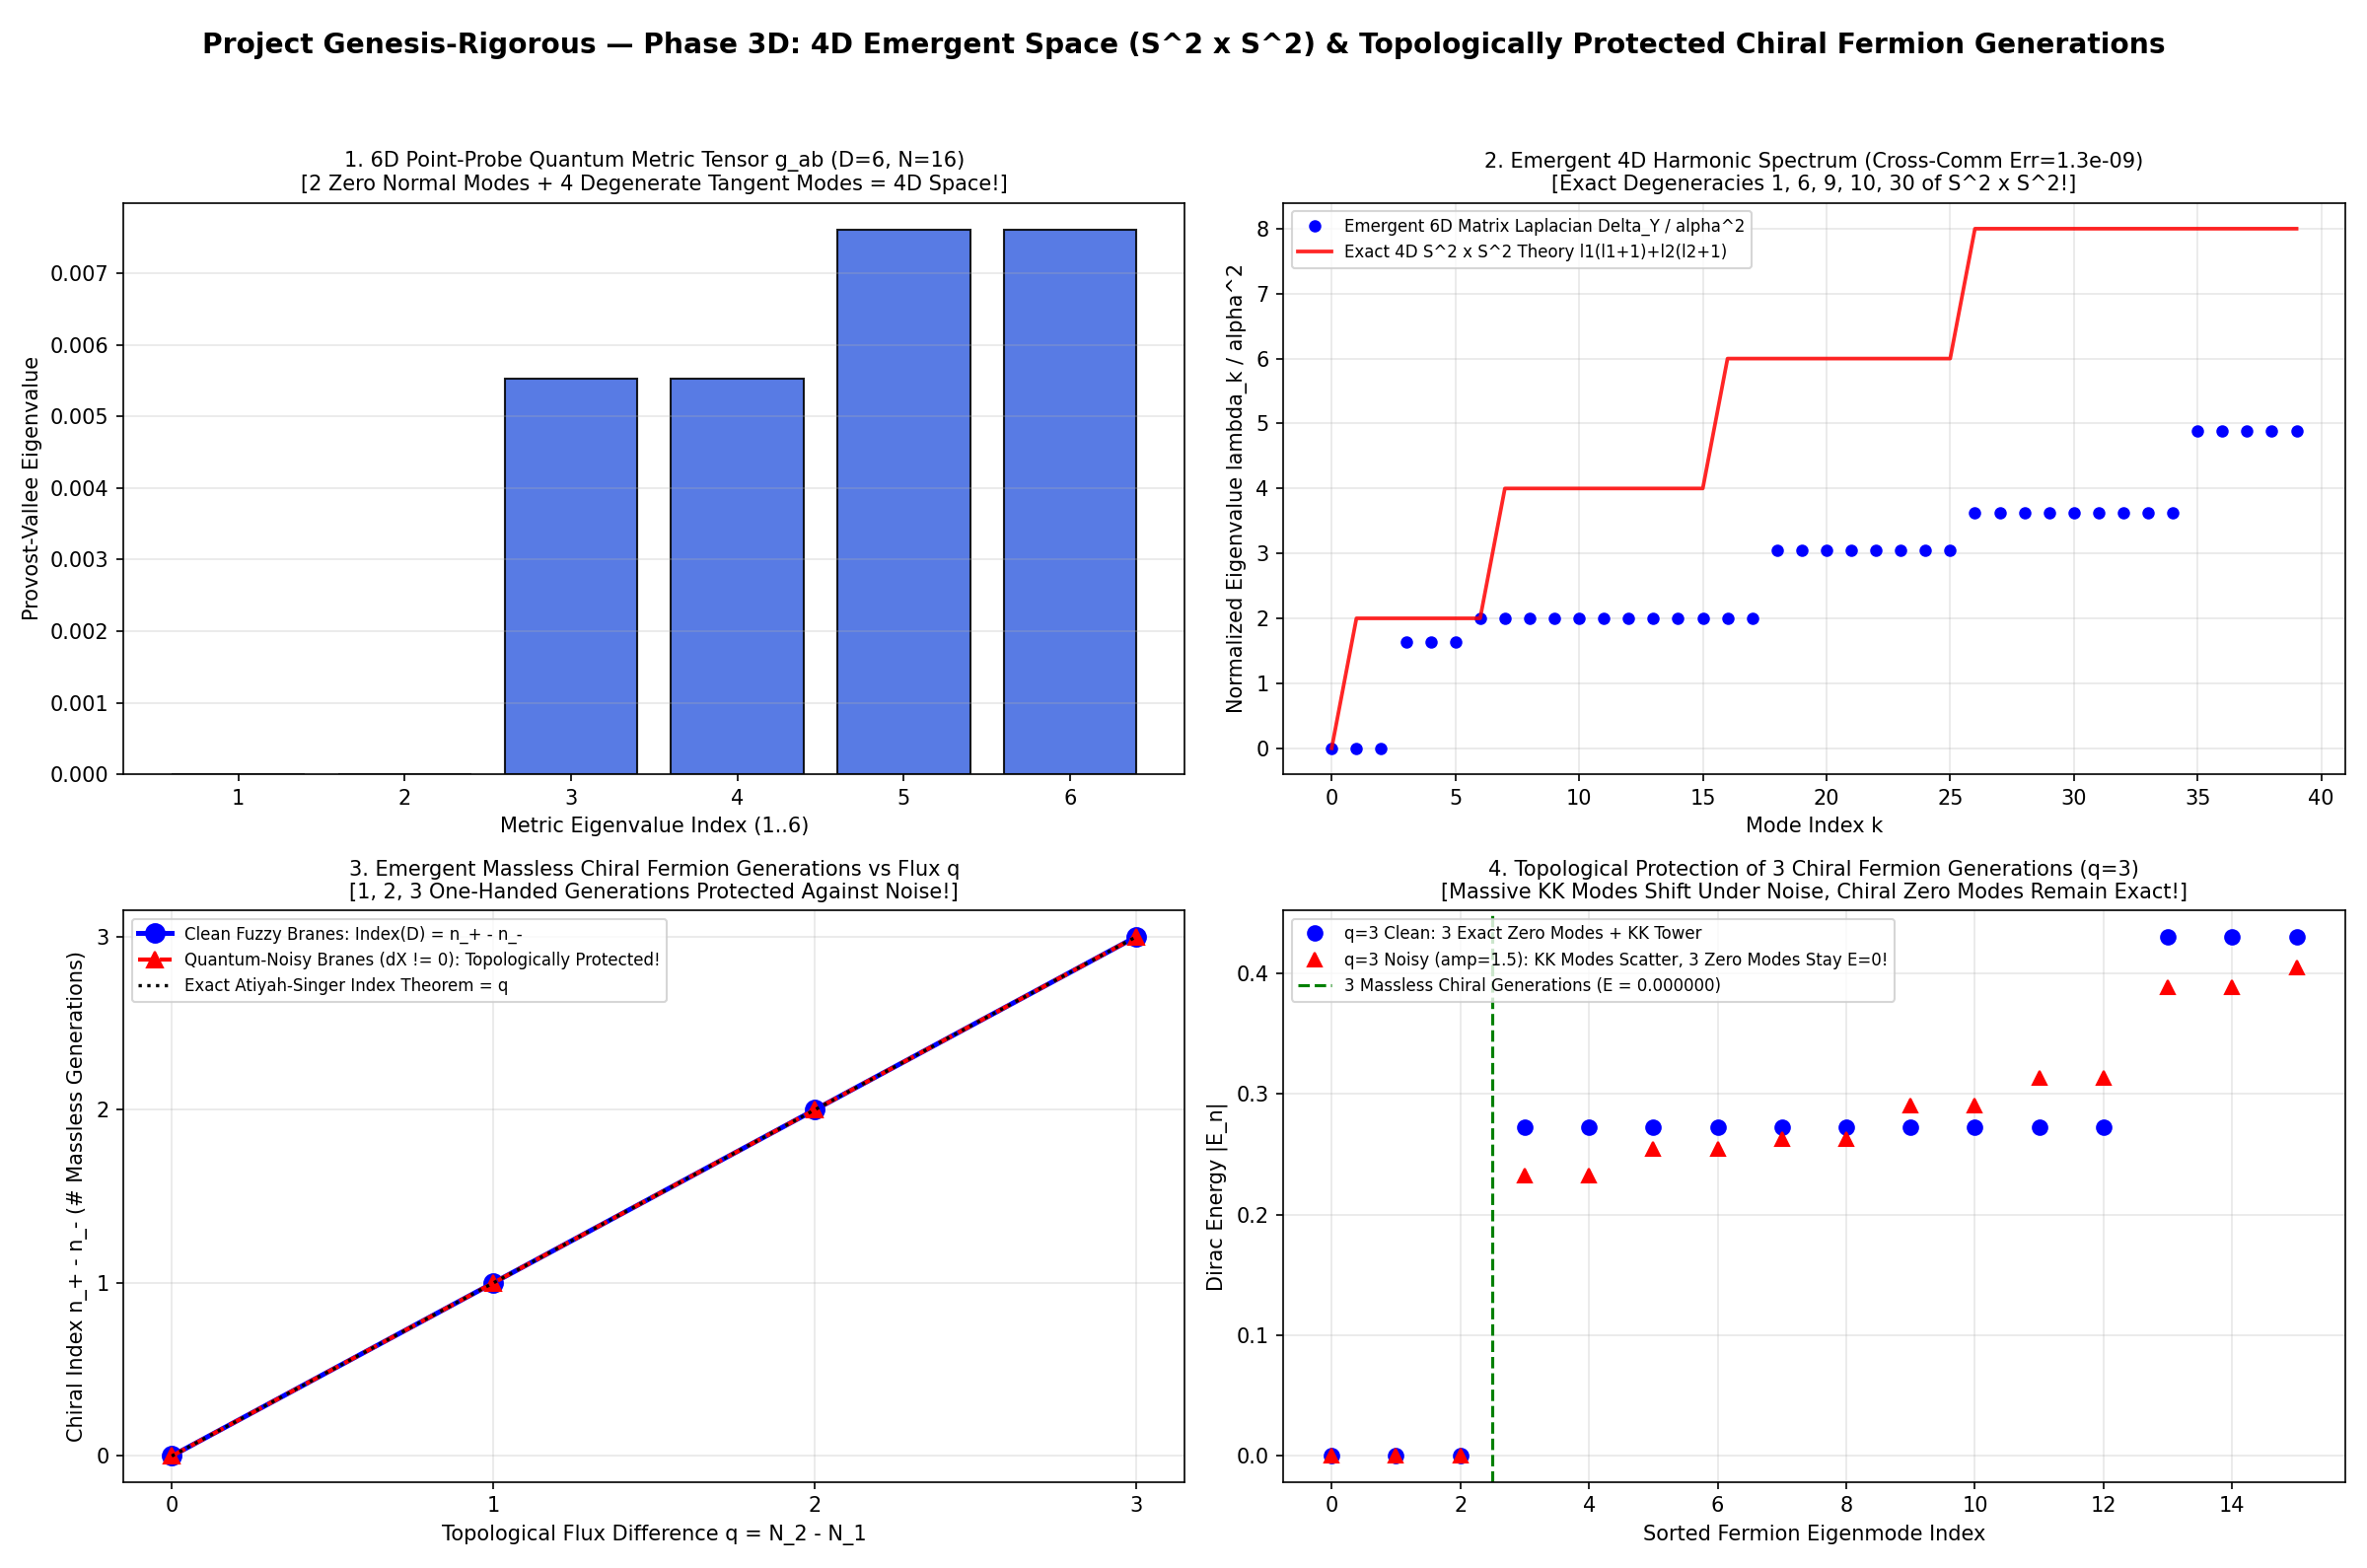
\includegraphics[width=\textwidth]{figures/fig7_phase3d_4d_chiral.png}
  \caption{Phase~3D four-dimensional emergent space and topologically protected chiral fermions (archival run \texttt{phase3d\_4d\_chiral\_20261125\_182622}). Left: 6D Provost--Vall\'ee quantum metric spectrum demonstrating exact rank-4 geometry ($S^2\times S^2$) with two vanishing normal eigenvalues. Right: topological protection of $q=3$ massless chiral generations at $|E_0|\le 7\times 10^{-16}$ despite strong matrix noise scattering the massive Kaluza--Klein tower.}
  \label{fig:phase3d}
\end{figure}

% ==============================================================================
\section{Discussion, Limitations, and Scientific Scope Boundaries}
\label{sec:discussion}
% ==============================================================================

A central goal of this work is to distinguish clearly between what is rigorously demonstrated inside this computational testbed and what lies beyond its physical or numerical scope. Five specific limitations merit explicit attention:

\begin{enumerate}
  \item \textbf{HFB Gaussian truncation versus non-perturbative quantum fluctuations.}
  The bosonic sector is treated within self-consistent Hartree--Fock--Bogoliubov (Gaussian) wave-packets. While HFB captures one-loop fluctuation pressure, zero-point energy renormalization ($\alpha(N) < \alpha_{\mathrm{cl}}$), and exact Gaussian bosonic entanglement, it cannot describe macroscopic quantum tunneling between distinct $SU(2)$ topological sectors (such as the $3\oplus 5$ metastable multi-sphere and the $N=8$ global sphere), nor strongly non-Gaussian matrix liquids at very large coupling $g$. Comparing HFB against neural VMC~\cite{Han2020} or hybrid Monte Carlo at matched parameters remains an informative next step.

  \item \textbf{Single-particle coherent Dirac backreaction versus full fermionic determinant.}
  In Stage~3 and Phase~3A, localized matter is modeled by the spin-averaged positive-energy expectation value $E_{\mathrm{matter}}(Y)$ of Eq.~\eqref{eq:Ematter} rather than a full second-quantized fermion determinant $\det(\mathcal{D}_{\mathrm{adj}})$ or occupied Dirac sea. This choice preserves strict $U(N)$ gauge invariance and avoids UV Dirac-sea dominance at finite $N$, cleanly isolating localized single-particle backreaction, but it does not incorporate vacuum polarization loops from dynamical adjoint fermions or pair creation during rapid real-time pulses.

  \item \textbf{Fixed-width linear-response real-time evolution.}
  In Phase~3A-2, symplectic Velocity--Verlet integration evolves the matrix means and momenta $(Y(t), P(t))$ with the HFB covariance $\Sigma_x^*$ held fixed at its static equilibrium value, while keeping the BdG and Dirac gradients fully dynamic. Integrating the complete time-dependent HFB matrix Riccati equations for $(\Sigma_x(t), \Sigma_p(t))$ would include dynamical squeezing and quantum-noise radiation during wave propagation and is left for future work.

  \item \textbf{Nature of emergent gravity in $(0+1)$D bosonic MQM.}
  The gravitational phenomena reproduced in Stage~3 and Phase~3A---positive intrinsic Gaussian curvature concentration, area contraction reminiscent of a $(2+1)$D conical deficit angle, minimal-surface repulsion, and a Yukawa-screened attractive two-body potential---reflect the elastic/curvature response of a finite-$N$, noncommutative 2D fuzzy-brane worldvolume with massive radial breathing modes. They do \emph{not} constitute massless $(3+1)$-dimensional spin-2 Einstein--Hilbert graviton propagation or Lorentz-invariant 4D cosmology. Likewise, our 4D $S^2\times S^2$ stabilization relies on an explicit doubled-Myers plus $\phi^4$ potential and does not address the dynamical $SO(9)\to SO(3)$ symmetry-breaking / complex-phase sign problem of the 10D supersymmetric IKKT model~\cite{Ishibashi1997}, nor the Yukawa mass hierarchies of the Standard Model.

  \item \textbf{Finite-$N$ optimization landscape.}
  As documented transparently in Sections~\ref{sec:exp_phase1} and~\ref{sec:exp_largeN}, unconstrained gradient relaxation from random GUE initializations naturally encounters physical local minima: concentric multi-spheres ($3\oplus 5$ at $N=8$; reducible basins at $N=20, 24$ under a 3-seed budget) and equatorial two-circle saddles in single-start Grassmannian entanglement minimization ($N=10, 12$). Rather than hiding these basins behind heuristic initializations, future extensions should pair the $O(N^3)$ engine with parallel tempering or multi-start Riemannian conjugate-gradient solvers on the Grassmannian.
\end{enumerate}

% ==============================================================================
\section{Software Availability and Reproducibility}
\label{sec:repro}
% ==============================================================================

The complete modular Python/PyTorch implementation (\texttt{Genesis-Rigorous v1.0.0}), automated 17-test audit suite, curated benchmark JSON/PNG artifacts, and reproducible state checkpoints are archived permanently on Zenodo under the MIT License (\href{https://doi.org/10.5281/zenodo.24528178}{\texttt{DOI:10.5281/zenodo.24528178}}). After installing dependencies (\texttt{pip install -r requirements.txt}), all verifications and experiments can be reproduced directly via the unified command-line interface:
\begin{verbatim}
python -m unittest discover -s tests -v                  # 17-test mathematical audit (~2 s)
python genesis_cli.py phase1 --N 8                       # Phase 1 emergence & blind area law
python genesis_cli.py gravity                            # Stage 3 adjoint Dirac backreaction
python genesis_cli.py realtime                           # Phase 3A 2-body gravity & light cone
python genesis_cli.py large-n --Ns 16,20,24,32           # Phase 3B O(N^3) continuum scaling
python genesis_cli.py gauge --n-sphere 6                 # Phase 3C U(2) Higgs bosons
python genesis_cli.py chiral                             # Phase 3D 4D S^2 x S^2 & chiral modes
python genesis_cli.py suite --fast                       # End-to-end showcase suite (~100 s)
\end{verbatim}
All experiments incorporate hardware preflight memory checks (\texttt{HardwareSafetyGuard}) to prevent out-of-memory failures and run comfortably on any CUDA-capable GPU with $\ge 2$~GB VRAM (or CPU fallback for smaller $N$).

\bibliographystyle{unsrt}
\bibliography{references}

\end{document}
